%Fred's NSF Grant Dec 2018
% GitHub: https://github.com/fjhickernell/NSF_CompMath2018Nov
% Overleaf: https://www.overleaf.com/9576964687whkhbmrrvhsd
\documentclass[11pt]{NSFamsart}
\usepackage{latexsym,amsfonts,amsmath,epsfig,extdash,multirow}
\usepackage{stackrel,tabularx,mathtools,enumitem,xspace}
\usepackage[dvipsnames]{xcolor}
\usepackage[numbers]{natbib}
\usepackage{hyperref,accents, booktabs}
\usepackage{algorithm, algorithmicx}
\usepackage{anyfontsize}
\usepackage{cleveref}
\newcommand{\myshade}{85}
\colorlet{mylinkcolor}{violet}
\colorlet{mycitecolor}{Aquamarine}
%\colorlet{mycitecolor}{OliveGreen}
\colorlet{myurlcolor}{YellowOrange}

\hypersetup{
	linkcolor  = mylinkcolor!\myshade!black,
	citecolor  = mycitecolor!\myshade!black,
	urlcolor   = myurlcolor!\myshade!black,
	colorlinks = true,
}


% This package prints the labels in the margin
%\usepackage[notref,notcite]{showkeys}


%\pagestyle{empty}
\thispagestyle{plain}
\pagestyle{plain}

\headsep-0.6in
%\headsep-0.45in

%%list of acronyms with links
\newcommand{\QMCSoft}{\hyperlink{QMCSoftlink}{QMCSoft}\xspace}
\newcommand{\GAIL}{\hyperlink{GAILlink}{GAIL}\xspace}
\newcommand{\QMC}{\hyperlink{QMClink}{QMC}\xspace}
\newcommand{\IIDMC}{\hyperlink{IIDMClink}{IID MC}\xspace}
\newcommand{\SAMSIQMC}{\hyperlink{SAMSIlink}{SAMSI-QMC}\xspace}
\newcommand{\SciPy}{\hyperlink{SciPylink}{SciPy}\xspace}
\newcommand{\GSL}{\hyperlink{GSLlink}{GSL}\xspace}
\newcommand{\NAG}{\hyperlink{NAGlink}{NAG}\xspace}
\newcommand{\MATLAB}{\hyperlink{MATLABlink}{MATLAB}\xspace}
\newcommand{\Chebfun}{\hyperlink{Chebfunlink}{Chebfun}\xspace}
\newcommand{\Rlang}{\hyperlink{Rlink}{R}\xspace}
\newcommand{\Julia}{\hyperlink{Julialink}{Julia}\xspace}

\textwidth6.4in
\setlength{\oddsidemargin}{0in}
\setlength{\evensidemargin}{0in}
\textheight8.9in
%\textheight9.1in


\providecommand{\FJHickernell}{Hickernell}
\newcommand{\hf}{\widehat{f}}
\newcommand{\hg}{\widehat{g}}
\newcommand{\hI}{\hat{I}}
\newcommand{\hatf}{\hat{f}}
\newcommand{\hatg}{\hat{g}}
\newcommand{\tf}{\widetilde{f}}
\newcommand{\tbf}{\tilde{\bff}}
%\DeclareMathOperator{\Pr}{\mathbb{P}}
\DeclareMathOperator{\cost}{COST}
\DeclareMathOperator{\comp}{COMP}

\DeclareMathOperator{\loss}{loss}
\DeclareMathOperator{\lof}{lof}
\DeclareMathOperator{\reg}{reg}
\DeclareMathOperator{\CV}{CV}
\DeclareMathOperator{\size}{wd}
\DeclareMathOperator{\GP}{\mathcal{G} \! \mathcal{P}}
\DeclareMathOperator{\erf}{erf}


\newcommand{\reals}{{\mathbb{R}}}
\newcommand{\naturals}{{\mathbb{N}}}
\newcommand{\natzero}{{\mathbb{N}_0}}
\newcommand{\integers}{{\mathbb{Z}}}
\def\expect{{\mathbb{E}}}
\def\il{\left<}
\def\ir{\right>}
\def\e{\varepsilon}
\def\g{\gamma}
\def\l{\lambda}
\def\b{\beta}
\def\a{\alpha}
\def\lall{\Lambda^{{\rm all}}}
\def\lstd{\Lambda^{{\rm std}}}

\newcommand{\vf}{\boldsymbol{f}}
\newcommand{\hV}{\widehat{V}}
\newcommand{\tV}{\widetilde{V}}
\newcommand{\fu}{\mathfrak{u}}
\newcommand{\hcut}{\mathfrak{h}}
\newcommand{\tOmega}{\widetilde{\Omega}}
\newcommand{\tvarrho}{\widetilde{\varrho}}

\newcommand{\bbE}{\mathbb{E}}
\newcommand{\tQ}{\widetilde{Q}}
\newcommand{\mA}{\mathsf{A}}
\newcommand{\mB}{\mathsf{B}}
\newcommand{\mC}{\mathsf{C}}
\newcommand{\mD}{\mathsf{D}}
\newcommand{\mG}{\mathsf{G}}
\newcommand{\mH}{\mathsf{H}}
\newcommand{\mI}{\mathsf{I}}
\newcommand{\bbK}{\mathbb{K}}
\newcommand{\mK}{\mathsf{K}}
\newcommand{\tmK}{\widetilde{\mathsf{K}}}
\newcommand{\mL}{\mathsf{L}}
\newcommand{\mM}{\mathsf{M}}
\newcommand{\mP}{\mathsf{P}}
\newcommand{\mQ}{\mathsf{Q}}
\newcommand{\mR}{\mathsf{R}}
\newcommand{\mX}{\mathsf{X}}
\newcommand{\mPhi}{\mathsf{\Phi}}
\newcommand{\mPsi}{\mathsf{\Psi}}
\newcommand{\mLambda}{\mathsf{\Lambda}}
\newcommand{\cube}{[0,1]^d}
\newcommand{\design}{\{\bx_i\}_{i=1}^n}

\DeclareMathOperator{\err}{err}
\DeclareMathOperator{\oerr}{\overline{\err}}
\DeclareMathOperator{\herr}{\widehat{\err}}
\DeclareMathOperator{\Ans}{ANS}

\DeclareMathOperator{\Var}{Var}
\DeclareMathOperator{\SOL}{SOL}
\DeclareMathOperator{\APP}{APP}
\DeclareMathOperator{\ALG}{ALG}
\DeclareMathOperator{\ERR}{ERR}
\DeclareMathOperator{\OPER}{OPER}



\DeclareMathOperator{\INT}{INT}
\DeclareMathOperator{\OPT}{MIN}

\newcommand{\bone}{\boldsymbol{1}}
\newcommand{\bzero}{\boldsymbol{0}}
\newcommand{\binf}{\boldsymbol{\infty}}
\newcommand{\ba}{{\boldsymbol{a}}}
\newcommand{\bb}{{\boldsymbol{b}}}
\newcommand{\bc}{{\boldsymbol{c}}}
\newcommand{\bd}{{\boldsymbol{d}}}
\newcommand{\be}{{\boldsymbol{e}}}
\newcommand{\bff}{{\boldsymbol{f}}}
\newcommand{\bhh}{{\boldsymbol{h}}}
\newcommand{\beps}{{\boldsymbol{\varepsilon}}}
\newcommand{\tbeps}{\tilde{\beps}}
\newcommand{\bx}{{\boldsymbol{x}}}
\newcommand{\bX}{{\boldsymbol{X}}}
\newcommand{\bh}{{\boldsymbol{h}}}
\newcommand{\bj}{{\boldsymbol{j}}}
\newcommand{\bk}{{\boldsymbol{k}}}
\newcommand{\bg}{{\boldsymbol{g}}}
\newcommand{\bn}{{\boldsymbol{n}}}
\newcommand{\bv}{{\boldsymbol{v}}}
\newcommand{\bu}{{\boldsymbol{u}}}
\newcommand{\by}{{\boldsymbol{y}}}
\newcommand{\bt}{{\boldsymbol{t}}}
\newcommand{\bz}{{\boldsymbol{z}}}
\newcommand{\bvarphi}{{\boldsymbol{\varphi}}}
\newcommand{\bgamma}{{\boldsymbol{\gamma}}}
\newcommand{\bphi}{{\boldsymbol{\phi}}}
\newcommand{\bpsi}{{\boldsymbol{\psi}}}
\newcommand{\bnu}{{\boldsymbol{\nu}}}
\newcommand{\balpha}{{\boldsymbol{\alpha}}}
\newcommand{\bbeta}{{\boldsymbol{\beta}}}
\newcommand{\bo}{{\boldsymbol{\omega}}}  %GF added
\newcommand{\newton}[2]{\left(\begin{array}{c} #1\\ #2\end{array}\right)}
\newcommand{\anor}[2]{\| #1\|_{\mu_{#2}}}
\newcommand{\satop}[2]{\stackrel{\scriptstyle{#1}}{\scriptstyle{#2}}}
\newcommand{\setu}{{\mathfrak{u}}}

\newcommand{\me}{\textup{e}}
\newcommand{\mi}{\textup{i}}
\def\d{\textup{d}}
\def\dif{\textup{d}}
\newcommand{\cc}{\mathcal{C}}
\newcommand{\cb}{\mathcal{B}}
\newcommand{\cl}{L}
\newcommand{\ct}{\mathfrak{T}}
\newcommand{\cx}{{\Omega}}
\newcommand{\cala}{{\mathcal{A}}}
\newcommand{\calc}{{\mathcal{C}}}
\newcommand{\calf}{{\mathcal{F}}}
\newcommand{\calfd}{{\calf_d}}
\newcommand{\calh}{{\mathcal{H}}}
\newcommand{\tcalh}{{\widetilde{\calh}}}
\newcommand{\calI}{{\mathcal{I}}}
\newcommand{\calhk}{\calh_d(K)}
\newcommand{\calg}{{\mathcal{G}}}
\newcommand{\calgd}{{\calg_d}}
\newcommand{\caln}{{\mathcal{N}}}
\newcommand{\cL}{\mathcal{L}}
\newcommand{\cP}{\mathcal{P}}
\newcommand{\cT}{\mathcal{T}}
\newcommand{\cK}{\mathcal{K}}
\newcommand{\fA}{\mathfrak{A}}
\newcommand{\fC}{\mathfrak{C}}
\newcommand{\fF}{\mathfrak{F}}
\newcommand{\fL}{\mathfrak{L}}
\newcommand{\fU}{\mathfrak{U}}
\newcommand{\hS}{\widehat{S}}
\DeclareMathOperator{\Prob}{\mathbb{P}}

\def\abs#1{\ensuremath{\left \lvert #1 \right \rvert}}
\newcommand{\bigabs}[1]{\ensuremath{\bigl \lvert #1 \bigr \rvert}}
\newcommand{\norm}[2][{}]{\ensuremath{\left \lVert #2 \right \rVert}_{#1}}
\newcommand{\ip}[3][{}]{\ensuremath{\left \langle #2, #3 \right \rangle_{#1}}}
\newcommand{\bignorm}[2][{}]{\ensuremath{\bigl \lVert #2 \bigr \rVert}_{#1}}
\newcommand{\calm}{{\mathfrak{M}}}
\DeclareMathOperator{\diag}{diag}
\DeclareMathOperator{\dist}{dist}
\DeclareMathOperator{\filldis}{fill}
\DeclareMathOperator{\sep}{sep}
\DeclareMathOperator{\avg}{avg}
\DeclareMathOperator{\vol}{vol}
\DeclareMathOperator{\cov}{cov}

\newcommand{\des}{\{\bx_i\}}
\newcommand{\desinf}{\{\bx_i\}_{i=1}^{\infty}}
\newcommand{\desn}{\{\bx_i\}_{i=1}^n}
\newcommand{\wts}{\{g_i\}_{i=1}^N}
\newcommand{\wtsn}{\{g_i\}_{i=1}^N}
\newcommand{\datan}{\{y_i\}_{i=1}^N}

%FJH added
\newcommand{\Order}{\mathcal{O}}
\newcommand{\ch}{\mathcal{H}}
\newcommand{\tch}{{\widetilde{\ch}}}
\newcommand{\veps}{\boldsymbol{\varepsilon}}
\DeclareMathOperator{\best}{best}
\newcommand{\hmu}{\hat{\mu}}
\newcommand{\hsigma}{\hat{\sigma}}
\newcommand{\tK}{\widetilde{K}}
%\newcommand{\Matlab}{{\sc Matlab}\xspace}
\newcommand{\abstol}{\varepsilon_{\text{a}}}
\newcommand{\reltol}{\varepsilon_{\text{r}}}

\newcommand\starred[1]{\accentset{\star}{#1}}

\newcommand{\designInf}{\{\bx_i\}_{i=1}^\infty}
\newcommand{\dataN}{\bigl\{\bigl(\bx_i,f(\bx_i)\bigr)\bigr\}_{i=1}^n}
\newcommand{\dataNp}{\bigl\{\bigl(\bx_i,f(\bx_i)\bigr)\bigr\}_{i=1}^{n'}}
\newcommand{\dataNo}{\bigl\{\bigl(\bx_i,f(\bx_i)\bigr)\bigr\}_{i=1}^{n_0}}
\newcommand{\ErrN}{\ERR\bigl(\dataN,n\bigr)}
\newcommand{\fint}{f_{\text{int}}}
\newcommand{\inflate}{\fC}


\definecolor{MATLABOrange}{rgb}{0.85,  0.325, 0.098}

%\newtheorem{resproblem}{Research Problem}
%\newtheorem{research}{Research Objectives}



%\setcounter{page}{1}
\usepackage{algpseudocode}
\algnewcommand\algorithmicparam{\textbf{Parameters:}}
\algnewcommand\PARAM{\item[\algorithmicparam]}
\algnewcommand\algorithmicinput{\textbf{Input:}}
\algnewcommand\INPUT{\item[\algorithmicinput]}
%\algnewcommand\STATE{\item}
\algnewcommand\RETURN{\State \textbf{Return }}


\setlist[description]{font=\normalfont\itshape}

\makeatletter
\newenvironment{varsubequations}[1]
 {%
  \addtocounter{equation}{-1}%
  \begin{subequations}
  \renewcommand{\theparentequation}{#1}%
  \def\@currentlabel{#1}%
 }
 {%
  \end{subequations}\ignorespacesafterend
 }
\makeatother


%\newcommand{\smallerscoop}{\includegraphics[width=0.7cm]{ProgramsImages/IceCreamScoop.eps}\xspace}
\newcommand{\smallerscoop}{\parbox{0.7cm}{\includegraphics[width=0.7cm]{ProgramsImages/IceCreamScoop.eps}}\xspace}
\newcommand{\smallscoop}{\parbox{1cm}{\includegraphics[width=1cm]{ProgramsImages/IceCreamScoop.eps}}\xspace}
\newcommand{\medscoop}{\parbox{1.8cm}{\includegraphics[width=1.8cm]{ProgramsImages/IceCreamScoop.eps}}\xspace}
\newcommand{\meddanger}{\parbox{0.8cm}{\vspace{-0.3cm}\includegraphics[width=0.75cm]{ProgramsImages/dangersign.eps}}\xspace}
\newcommand{\medcone}{\parbox{1.2cm}{\includegraphics[width=0.55cm,angle=270]{ProgramsImages/MediumWaffleCone.eps}}\xspace}
\newcommand{\largercone}{\parbox{2.2cm}{\vspace*{-0.2cm}\includegraphics[width=1cm,angle=270]{ProgramsImages/MediumWaffleCone.eps}}\xspace}
\newcommand{\largecone}{\parbox{1.54cm}{\vspace*{-0.2cm}\includegraphics[width=0.7cm,angle=270]{ProgramsImages/MediumWaffleCone.eps}}\xspace}
\newcommand{\smallcone}{\parbox{0.7cm}{\includegraphics[width=0.32cm,angle=270]{ProgramsImages/MediumWaffleCone.eps}}\xspace}




\begin{document}
%\setlength{\leftmargini}{2.5ex}

\centerline{\Large \textbf{Project Description}}
\vspace{-2ex}

\setcounter{tocdepth}{1}
\tableofcontents

\vspace{-6ex}

%%%%%%%%%%%%%%%%%%%%%%%%%%%%%%%%%%%%%%%%%%%%%%%%%%%%
\section{Scientific Context, Key Ideas, and Timeliness of the Proposed Research}
%%%%%%%%%%%%%%%%%%%%%%%%%%%%%%%%%%%%%%%%%%%%%%%%%%%%

Integration and function approximation are key to
solving practical problems in a variety of areas, including financial risk management~\cite{Gla03}, 
statistical physics~\cite{LanBin14}, 
Bayesian inference~\cite{GelEtal13}, and uncertainty quantification~\cite{ForEtal09, Smi14a}.  As computational mathematicians, we should provide rigorously justified algorithms that satisfy practitioners.  They want algorithms that 
\begin{enumerate}[leftmargin = 15ex]
\renewcommand{\labelenumi}{\textbf{Goal \arabic{enumi}.}}

\item \label{GoalOne} Meet their error criteria,
    
\item \label{GoalTwo} Require minimal a priori knowledge about the input function,

\item \label{GoalThree} Are computationally efficient,

\item \label{GoalFour} Are readily available and easy to use, and

\item \label{GoalFive} Work well in practice.
\end{enumerate}
We, the PIs, Choi (SCTC) and Hickernell (FJH), will construct algorithms that meet those goals.

Some research on multivariate integration and function approximation focuses on solid theory and ignores whether it is relevant to applications.  Other research focuses on constructing practical algorithms, even if they are based on heuristics.  \emph{We propose to provide practical algorithms based on sound theory.}  What we may sacrifice initially is tackling more difficult mathematical problems.  We focus on relatively simpler settings where Goals 1--5 can be attained. However, we expect our efforts to inspire similar research for sound, practical algorithms in other settings.  Because our paradigm is uncommon, we spend a significant portion of this project description explaining it.

%%%%%%%%%%%%%%%%%%%%%%%%%%%%%%%%%%%%%%%%%%%%%%%%%%%%
\subsection{Problems to be Solved} \label{sec:Problems}
%%%%%%%%%%%%%%%%%%%%%%%%%%%%%%%%%%%%%%%%%%%%%%%%%%%%

The mathematical problems to solve take the form 
%\begin{subequations} \label{problem}
\begin{align*}
    \calf & = \text{a Banach space of inputs functions}, \qquad 
    \calg = \text{a Banach space of outputs}, \\
    \SOL : \calf  \to \calg & = \text{ a linear solution operator} \\
    \nonumber
    \MoveEqLeft[6]{\text{e.g., integration }\SOL(f) := \int_{\cube} f(\bx) \, \dif \bx
    \qquad \text{or function approximation } \SOL(f) = f.}
\end{align*}
%\end{subequations}
There often already exist approximate solutions requiring $n$ function values at well-chosen node sets, $\design$, which take the form
\begin{equation}
    \APP: \calf \times \naturals_0 \to \calg = \text{fixed sample size approximation}, \quad \APP(f,n) = \sum_{i=1}^n f(\bx_i) g_i, \ \ g_i \in \calg.
\end{equation}
For integration, the $g_i$ are real-valued weights, which are generally equal for (quasi\Hyphdash*)Monte Carlo methods but unequal for Newton-Cotes, Gauss, or Bayesian quadratures or cubatures.  For function approximation, the $g_i$ are cardinal functions that arise from a (piece-wise) polynomial or kriging approximation. We define $\APP(f,0) = 0$.

To meet Goal \ref{GoalOne} we need error bounds, which often take the form
\begin{equation}  \tag{ERR-BD} \label{errorBd}
    \norm[\calg]{\SOL(f) - \APP(f,n)} \le \norm[\calf \to \calg]{\SOL(\cdot) - \APP(\cdot,n)} \, \norm[\calf]{f} \quad \forall f\in \calf, \ n \in \naturals,
\end{equation}
where $\norm[\calf \to \calg]{\SOL(\cdot) - \APP(\cdot,n)}$ is the norm of the error operator.  Here, $\norm[\calf]{\cdot}$ is a (semi-)norm.  As an example, for the composite trapezoidal rule $\norm[\calf]{f}$ could be the total variation of $f'$, in which case $\norm[\calf \to \calg]{\SOL(\cdot) - \APP(\cdot,n)} = 1/[8 (n-1)^2]$ \cite[Sect.\ 7.2, (7.15)]{BraPet11a}.  Even when the norm of the error operator has an explicit expression or upper bound, $\norm[\calf]{f}$ is typically unknown a priori.  Therefore, error bound \eqref{errorBd} is insufficient to satisfy Goal \ref{GoalOne}. 

%%%%%%%%%%%%%%%%%%%%%%%%%%%%%%%%%%%%%%%%%%%%%%%%%%%%
\subsection{Adaptive Algorithms} \label{sec:AdapAlgo}
%%%%%%%%%%%%%%%%%%%%%%%%%%%%%%%%%%%%%%%%%%%%%%%%%%%%

Goal \ref{GoalOne} requires an algorithm of the form
\begin{equation*}
    \ALG : \calf \times (0,\infty) \to \calg = \text{fixed error tolerance algorithm},
\end{equation*}
which satisfies the error criterion
\begin{equation}
      \tag{ALG-CRIT} \label{AlgErr}
    \norm[\calg]{\SOL(f) - \ALG(f,\varepsilon)} \le \varepsilon \quad \text{(with high probability)} \qquad \forall f\in \calc, \ \varepsilon >0.
\end{equation}
Here $\calc$ is a well-chosen subset of $\calf$ for which $\ALG$ can be proven to succeed.  The user need only specify the error tolerance, $\varepsilon$, and is freed from having to choose the appropriate $n$.  The computational cost is determined by the accuracy requirement (see Sect.\ \ref{sec:CompEff}).  If the algorithm is random, we will accept that it satisfies the error tolerance with high probability.  

Algorithms satisfying \eqref{AlgErr} use approximations satisfying \eqref{errorBd} combined with a \emph{stopping criterion} that adaptively determines the sample size.  $\ALG$ requires a \emph{data-driven error bound}, which depends on the definition of $\calc$ and on the function data required by $\APP(f,n)$:
%\begin{subequations}\label{dataErrBdStop}
\begin{multline} \label{dataErrBd} \tag{DATA-BD}
\norm[\calg]{\SOL(f) - \APP(f,n)} \le \ErrN \quad \text{(with high probability)} \\ \forall f \in \cc, \ n \in \naturals.
\end{multline}
The stopping criterion is then
\begin{equation} \label{stopCrit} \tag{STOP}
\ALG(f,\varepsilon) = \APP(f,n^*) \quad \text{for } n^* = \min \left \{ n : \ErrN \le \varepsilon \right \}.
\end{equation}
%\end{subequations}
The values of $n$ for which the error bound is evaluated are typically only some subset of positive integers, e.g., powers of two.  While there is a substantial literature on approximations with theoretical error bounds \eqref{errorBd}, the construction of data-driven error bounds that satisfy \eqref{dataErrBd} has been neglected. 

%%%%%%%%%%%%%%%%%%%%%%%%%%%%%%%%%%%%%%%%%%%%%%%%%%%%
\subsection{Existing Adaptive Algorithms Typically Employ Heuristic Stopping Criteria} \label{sec:Heuristics}
%%%%%%%%%%%%%%%%%%%%%%%%%%%%%%%%%%%%%%%%%%%%%%%%%%%%

The demand for algorithms satisfying Goal \ref{GoalOne} is evidenced by the automatic quadrature, function approximation, optimization, and root-finding algorithms found in widely used software.  Examples include \hypertarget{MATLABlink}{MATLAB}'s \cite{MAT9.5} native \texttt{integral}, \texttt{fminbnd}, and \texttt{fzero} algorithms.  The \hypertarget{Chebfunlink}{Chebfun} \MATLAB library \cite{TrefEtal17a} adaptively approximates $f$ by Chebyshev polynomials and then overloads \MATLAB's \texttt{sum}, \texttt{cumsum}, \texttt{min}, and \texttt{roots} functions to approximate definite integrals, indefinite integrals, minima, and zeros of $f$.  The  Numerical Algorithms Group
(\hypertarget{NAGlink}{NAG}) library \citep{NAG23}, the Python scientific library \hypertarget{SciPylink}{SciPy} \cite{SCIPY}, and the GNU Scientific Library (\hypertarget{GSLlink}{GSL}) \cite{GSL} have automatic quadrature and cubature. 

\newlength{\figwidthA}
\setlength{\figwidthA}{0.45\textwidth}
\newlength{\figheightB}
\setlength{\figheightB}{0.2\textwidth}
\begin{figure}[h]
	\begin{tabular}{>{\centering}m{\figwidthA}@{\qquad}>{\centering}m{\figwidthA}}
		\includegraphics[height=\figheightB]{ProgramsImages/SpikyFoolIntegralcolor.eps} &
		\includegraphics[height=\figheightB]{ProgramsImages/FlukyFoolIntegralcolor.eps} 
		\tabularnewline
		a) $\abs{\SOL(f) - \ALG(f,1\text{E}{-14})} = 1 $ &
		b) $\abs{\SOL(f) - \ALG(f,1\text{E}{-14})} =  2.8\text{E}{-5}$
		\end{tabular}
	\caption{Integrands for which MATLAB's \texttt{integral} fails. \label{quadfailfig}}
\end{figure}

All of these algorithms, and others like them, fail to satisfy the error tolerance if the input function is sufficiently spiky.  Fig.\ \ref{quadfailfig}a) depicts a spiky integrand that fools \MATLAB's \texttt{integral}.  Although $\SOL(f) = \int_0^1 f(x) \, \dif x = 1$, $\ALG(f,1\text{E}{-14}) = \texttt{integral}(f,1\text{E}{-14}) = 0$, and the error of $1$ is significantly greater than the tolerance of $1\text{E}{-14}$.  Any algorithm relying on function values may be fooled by sufficiently spiky functions.  However, the algorithms mentioned above \emph{have no theory} that specifies the set of input functions, $\calc$, for which they must succeed.

A data-driven error bound \eqref{dataErrBd}---needed for Goal \ref{GoalOne}---requires $\calc$ to \emph{exclude} spiky functions.  This is why $\calc$ is a strict subset of the input space $\calf$.

Spiky inputs are not the only source of failure for adaptive quadratures. 
\MATLAB's state-of-the-art
\texttt{integral} \cite{Sha08a, MAT9.5} estimates the quadrature error based on the difference between two different Gauss quadratures with nodes. This flawed way of estimating error was criticized by 
Lyness \cite[p.\ 69]{Lyn83} over 30 years ago.  Lyness claimed that automatic quadratures employing this type of error estimate are ``\ldots likely to be unreliable in a significant proportion of the problems it faces 
	(say $1$ to $5\%$) and there is no way of predicting in a straightforward way in which of any set
	of apparently reasonable problems this will happen.''
Fig.\ \ref{quadfailfig}b) displays a fluky integrand for which \MATLAB's \texttt{integral} fails to meet the specified error tolerance.  It does not fail because of integrand fluctuations between the nodes.  Rather it fails because the two Gauss quadratures give the same \emph{wrong} answer.  Other common adaptive quadratures fail similarly.  In contrast, the adaptive quadrature developed by the FJH and collaborators \cite{HicEtal14b, Zha18a}, which follows the procedure described above and is highlighted in Sect.\ \ref{sec:localadpat}, is not fooled by fluky integrands.



There is a family of theoretically justified, adaptive algorithms based on \emph{interval 
arithmetic} described in \cite{MoKeCl09} and \cite{Rum10a} and implemented in INTLAB 
\cite{Rum99a}.  This approach requires the function routines to take \emph{interval} arguments 
and return \emph{interval} outputs.  We do not pursue this approach because existing black-box 
function routines normally do not meet these requirements.

%%%%%%%%%%%%%%%%%%%%%%%%%%%%%%%%%%%%%%%%%%%%%%%%%%%%
\subsection{The Choice of $\calc$} \label{sec:CChoice}
%%%%%%%%%%%%%%%%%%%%%%%%%%%%%%%%%%%%%%%%%%%%%%%%%%%%

The de facto choice for many is to let $\calc$ be a ball, $\cb_{\rho} := \{f \in \calf : \norm[\calf]{f} \le \rho \}$, which resembles a scoop of ice cream, \smallerscoop.  Then one may construct $\ALG$ satisfying \eqref{AlgErr} as in Algorithm \ref{BallAlg}. \emph{Parameters} are set by the algorithm designer and essentially unchanged e.g., the initial sample sizes in \MATLAB's \texttt{integral} and the \Chebfun library.  \emph{Inputs} are provided by the user and likely change each time the algorithm is called.

\begin{algorithm}
	\caption{Model Ball-Based $\ALG$ \label{BallAlg}} 
	\begin{algorithmic}
	\PARAM a radius, $\rho$; $\APP$ satisfying \eqref{errorBd}
		\INPUT a black-box function, $f$; an absolute error tolerance,
		$\varepsilon>0$

\Ensure \eqref{AlgErr} for $\cc = \cb_{\rho}$\smallerscoop

\State Choose $\ErrN = \norm[\calf \to \calg]{\SOL(\cdot) - \APP(\cdot,n)} \rho$ \Comment{to satisfy \eqref{dataErrBd}}

\State Choose $n^*$ according to \eqref{stopCrit}

\RETURN $\ALG(f,\varepsilon) = \APP(f,n^*)$
\end{algorithmic}
\end{algorithm}

\begin{algorithm}
	\caption{Model Cone-Based $\ALG$ \label{ConeAlg}} 
	\begin{algorithmic}
	\PARAM an initial sample size, $n_0$; an inflation factor, $\fC$; $\APP$ satisfying \eqref{errorBd}
		\INPUT a black-box function, $f$; an absolute error tolerance,
		$\varepsilon>0$

\Ensure \eqref{AlgErr} for  the cone $\cc = \bigl\{f \in \calf : \norm[\calf]{f} \le \inflate \norm[\calf]{f_{\textup{int},n_0}} \bigr \}$\smallcone

\State Choose $\ErrN = \norm[\calf \to \calg]{\SOL(\cdot) - \APP(\cdot,n)} \inflate \norm[\calf]{f_{\textup{int},n_0}}$ \\ \Comment{satisfies \eqref{dataErrBd}}

\State Choose $n^* \ge n$ according to \eqref{stopCrit}

\RETURN $\ALG(f,\varepsilon) = \APP(f,n^*)$
\end{algorithmic}
\end{algorithm}


This ball-based algorithm is \emph{non-adaptive} because the error bound $\ErrN$ does not depend on the function data, but only on the parameter $\rho$ and on $n$.  To us, knowing a bound on the norm of your input function in advance violates Goal \ref{GoalTwo}.  

An \emph{adaptive} algorithm, whose computational cost depends on the input $f$, can be constructed for input functions whose norms are not much larger than their minimum norm interpolants.  Assume an infinite sequence of nodes, $\designInf$, and let $f_{\textup{int},n}$, denote the minimum norm interpolant of $f \in \calf$ based on the data $\dataN$.  Algorithm \ref{ConeAlg} is defined to succeed for a \emph{cone}, $\calc$, which resembles a waffle cone \smallcone.


Since the data-driven error bound, $\ErrN$, now actually depends on function data, this algorithm is adaptive.  The set $\calc$ is a cone because $f \in \calc$ implies $a f \in \calc$ for any real $a$.  The cone $\calc$ is defined by two parameters, the initial sample size and the inflation factor.  Increasing either makes the cone more inclusive and the algorithm more robust (and costly).  

The philosophy underlying Algorithm \ref{ConeAlg} is the following: \emph{what we do not observe about the input function is not much worse than what we observe}.  This rules out spiky functions, for which our algorithm will fail anyway.  Making this assumption allows us to satisfy Goal \ref{GoalTwo}.  We need not know too much about the function a priori; we learn it as we sample.

Algorithms designed to succeed for cones of inputs are typically more complex than those designed for balls of inputs, just as Algorithm \ref{ConeAlg} is more complex than Algorithm \ref{BallAlg}.  But, we assert that there are compelling advantages in defining the set of inputs for which our algorithms succeeds, $\calc$, as cones and not balls, or as a visual aid:

\centerline{  \largercone \qquad \qquad \medscoop \hspace{-11ex}\raisebox{-2.5ex}{\color{red}\fontsize{60}{72}\selectfont $\times$}
      }
\begin{itemize}
    \item Algorithms optimized for non-convex cones are often adaptive, whereas algorithms optimized for balls will not be.  Thus, easier problems take less computational effort than harder ones.  This helps us meet Goal \ref{GoalThree}.
    
    \item Having the initial sample size, $n_0$ and the inflation factor, $\inflate$, as rarely changed algorithm parameters is more intuitive than having the radius of the ball of inputs, $\rho$, as a rarely changed parameter, or even requiring the user to input it.  This helps us meet Goal \ref{GoalTwo}.
\end{itemize}

Algorithm \ref{ConeAlg} provides a paradigm for adaptive algorithms, which we have used in past NSF-funded research described in Sect.\ \ref{sec:Previous}.  However, this is not the whole story. In some cases $\norm[\calf \to \calg]{\SOL(\cdot) - \APP(\cdot,n)}$ and/or $\norm[\calf]{f_{\textup{int},n_0}}$ are computationally expensive, so alternative error bounds, $\ERR$, must be constructed.  How to do this is explained in Sects.\ \ref{sec:Previous} and \ref{sec:Proposed}.  Moreover, the cone $\calc$ in Algorithm \ref{ConeAlg} depends on the specific choice of nodes used $\APP$, which we want to avoid.  How we do this is also explained in Sects.\ \ref{sec:Previous} and \ref{sec:Proposed}.

%%%%%%%%%%%%%%%%%%%%%%%%%%%%%%%%%%%%%%%%%%%%%%%%%%%%
\subsection{How Do We Know that $f$ for Our Problem Is in the Cone $\calc$?} \label{sec:HowKnow}  
%%%%%%%%%%%%%%%%%%%%%%%%%%%%%%%%%%%%%%%%%%%%%%%%%%%%

Our answer to this frequent question is, ``We cannot know for sure.  The cone definition expresses prior beliefs.''  Similarly, we cannot know whether $f$ is in some ball, $\cb_{\rho}$.  We can be sure that if $\ALG(f,\varepsilon)$ fails to meet the error criterion, \eqref{AlgErr}, then $f$ lies outside $\calc$.  In this way we are pathologists, the doctors who determine why the patient has fallen sick or died.

More can be done.  In many cases there are data-driven necessary conditions that may alert the user that the input function lies outside the cone.  For example, in Algorithm \ref{ConeAlg}, $f \in \calc$ implies that $\norm[\calf]{f_{\textup{int},n^*}} \le \inflate \norm[\calf]{f_{\textup{int},n_0}}$.  If this does not hold, then one should make the cone more inclusive by increasing $\inflate$ and/or $n_0$.  In our existing and proposed adaptive algorithms,  we endeavor to derive such necessary conditions.

%%%%%%%%%%%%%%%%%%%%%%%%%%%%%%%%%%%%%%%%%%%%%%%%%%%%
\subsection{Computational Efficiency} \label{sec:CompEff}
%%%%%%%%%%%%%%%%%%%%%%%%%%%%%%%%%%%%%%%%%%%%%%%%%%%%

Goal \ref{GoalThree} requires our algorithm to use as little computation time or computational operations as possible.  We let $\cost(\ALG, f,\varepsilon)$ denote the \emph{information cost} of $\ALG$, i.e., the number of function data required by $\ALG(f,\varepsilon)$. To measure the overall performance of an algorithm, we define 
\begin{equation*}
    \cost(\ALG, \calc, \varepsilon,\rho) : = \max_{f \in \calc \cap \cb_{\rho}} \cost(\ALG,f,\varepsilon),
\end{equation*}
recognizing that this cost will generally increase as the norm of the input increases. Letting $\cala(\cc)$ denote the set of all possible algorithms, we define the \emph{computational complexity} of a problem as the information cost of the best algorithm:
\begin{equation*}
    \comp(\cala(\cc), \varepsilon,\rho) := \min_{\ALG \in \cala(\cc)} \cost(\ALG, \calc, \varepsilon,\rho) .
\end{equation*}
These definitions follow the information-based complexity literature \cite{TraWer98, TraWasWoz88}.
We define an algorithm to be essentially optimal if there exists some fixed positive $\omega$ for which
\begin{equation*}
    \cost(\ALG, \calc, \varepsilon,\rho) \le \comp(\cala(\cc), \omega \varepsilon,\rho) \qquad \forall \varepsilon,\rho > 0.
\end{equation*}
Part of Goal \ref{GoalThree} is to construct essentially optimal algorithms for $\calc$ that are cones, and not the balls, $\cb_{\rho}$, that have been studied in the past.

The $\varepsilon^{-1}$-dependence of $\cost(\ALG, \calc, \varepsilon,\rho)$ and $\comp(\cala(\cc), \varepsilon,\rho)$ is influenced by the input space, $\calf$.  If $\calf$ requires more smoothness, then the cost and complexity may grow more slowly with $\varepsilon^{-1}$.  For example, if $\calf$  assumes only finite variation of the first derivative, the complexity of univariate integration is $\Order(\varepsilon^{-1/2})$, but if $\calf$ assumes finite variation of the \emph{third} derivative, then the complexity of univariate integration is $\Order(\varepsilon^{-1/4})$.  The choice of approximation, $\APP$, also influences the information cost of $\ALG$.  For example, the composite trapezoidal rule can achieve $\Order(\varepsilon^{-1/2})$ cost for integrands whose first derivatives have finite variation but \emph{not} the optimal $\Order(\varepsilon^{-1/4})$ cost for integrands with sufficient smoothness.

Another aspect of Goal \ref{GoalThree} is to construct algorithms, $\ALG$, that can take advantage of additional smoothness to achieve low cost, but are still essentially optimal if the input, $f$, has only limited smoothness.  That is, we want \emph{a single} $\ALG$ that is smoothness adaptable.  It performs optimally across a spectrum of  $\calc$ with different smoothnesses.

Multivariate problems risk the \emph{curse of dimensionality}.  Let $f$ be a function of $d$ variables, and let's label the pieces of our problem, approximation, algorithm, etc.\ by $d$, i.e., 
\begin{equation*}
    \calf_d, \quad \calg_d, \quad \calc_d, \quad \SOL_d, \quad \APP_d,\quad \ALG_d, \quad \cala(\calc_d),
\end{equation*}
($\calg_d$ does not depend on $d$ for integration).  We want to know how $\cost(\ALG_d, \calc_d, \varepsilon,\rho)$ and $\comp(\cala(\cc_d), \varepsilon,\rho)$ depend on both $\varepsilon^{-1}$ and $d$.  This is the question of \emph{tractability}, an active area of recent research (see  Novak and Wo\'zniakowski \cite{NovWoz08a,NovWoz10a,NovWoz12a}).

Various flavors of tractability are defined in terms of how  $\comp(\cala(\cc_d), \varepsilon,\rho)$ grows with $d$.  By choosing appropriate norms for $\calf$ and $\calg$, we may often identify situations that avoid the curse of dimensionality (exponential growth in $d$) and even achieve strong tractability (independence of $d$).   For example, if the norms reflect that the importance of the variables, $x_1, x_2, \ldots$, decays quickly enough, which holds in many finance calculations, there is strong tractability.  Nearly all tractability studies assume that $\calc_d$ is a ball.  Goal \ref{GoalThree} involves determining the tractability of problems when $\calc_d$ is a cone.

If the information cost of $\ALG(f,\varepsilon)$ is $n^* = \cost(\ALG,f,\varepsilon)$, the cost of one $f(\bx)$ value is $\$_d(f)$, and the cost required by $\ALG(f,\varepsilon)$ to manipulate $\dataN$ is $\Order(n^{*p})$, then the total computational cost of $\ALG(f,\varepsilon)$ is $ \Order(\$_d(f)n^* + n^{*p})$.
Attaining the computational efficiency of Goal \ref{GoalThree} requires us to address several cases.  
\begin{description}

\item[Cheap Function Values]  If $\$_d(f)$ is small, then our algorithms should have $p \approx 1$ so that the cost of manipulating the function data does not dominate.  Probabilistic methods that model $f$ as a Gaussian process require matrix manipulations that ordinarily cost $\Order( n^{*3})$ (see Sects.\ \ref{sec:Bayes} and \ref{sec:NewBayes}).  We will find ways to avoid such costs.
    
    \item[Infinite $d$] When integrating functions of stochastic processes discretized by $d$ time steps, it is common to have $\$_d(f) = \Order(d)$ and to want the limit of the integral as $d \to \infty$.  Computational efficiency can be achieved by multi-level Monte Carlo methods and the multivariate domain decomposition method (Sect.\ \ref{sec:InfDim}).  

    \item[Expensive Function Values] In some practical  problems, such as constructing surrogates for expensive computer simulations,  $\$_d(f)$ is huge.  For practical reasons, $n^*$ must be moderate, say several hundred, and the cost of data manipulation is negligible---$p > 1$ is fine (Sect.\ \ref{sec:Expensive}).
\end{description}

%%%%%%%%%%%%%%%%%%%%%%%%%%%%%%%%%%%%%%%%%%%%%%%%%%%%
\subsection{Availability and Practicality} \label{sec:AvailPract}
%%%%%%%%%%%%%%%%%%%%%%%%%%%%%%%%%%%%%%%%%%%%%%%%%%%%

Practitioners rely on languages and software packages such as \MATLAB, \Chebfun, \NAG, \SciPy, \GSL, \hypertarget{Rlink}{R} \cite{R3.5.1_2018}, and \hypertarget{Julialink}{Julia} \cite{Julia1.0}. Whether commercial or open source, they are expected to provide reliable algorithms that have been carefully coded and tested.  

On the other hand, research code---which may provide significant advances over what is available in the above-mentioned software packages---is often difficult to access or use because authors have not invested the time to make it so.  Heeding the call for reproducible research \cite{BaiBor12a, Pen11, Sto14a} and better scientific software \cite{BSS18}, we will make our research code accessible, easy to use, and well tested.  We will continue the development of our Guaranteed Automatic Integration Library \hypertarget{GAILlink}{(GAIL)} \cite{ChoEtal17b}.  Moreover, we will combine our work with that of other research groups in a Quasi-Monte Carlo Community Software \hypertarget{QMCSoftlink}{(QMCSoft)}.  This will fulfill Goal \ref{GoalFour}.

Theory should not only be correct but also relevant to practical applications.  Making our software accessible and easy to use will facilitate others testing its practicality.  We will also try our algorithms on standard test cases, such as \cite{VirLib17a}.  This will fulfill Goal \ref{GoalFive}.

%%%%%%%%%%%%%%%%%%%%%%%%%%%%%%%%%%%%%%%%%%%%%%%%%%%%
\subsection{Remainder of This Project Description}
%%%%%%%%%%%%%%%%%%%%%%%%%%%%%%%%%%%%%%%%%%%%%%%%%%%%

More specifics of the ideas described above are provided below.  The next section describes results of a recently completed NSF grant.  Sect.\ \ref{sec:Proposed} describes the intellectual merit of our project.  Sect.\ \ref{SectBroad} describes the broader impact of our project.  FJH will take overall leadership of the project, especially the more theoretical portions.  SCTC will lead the software development efforts and assist in mentoring students.

%%%%%%%%%%%%%%%%%%%%%%%%%%%%%%%%%%%%%%%%%%%%%%%%%%%%
\section{Results of Previous NSF-Funded Research,
NSF-DMS-1522687\except{toc}{, \\ \emph{Stable, Efficient, Adaptive Algorithms for 
Approximation and 
Integration}, \\
\$270,000, August 2015 -- July 2018}} \label{sec:Previous}
%%%%%%%%%%%%%%%%%%%%%%%%%%%%%%%%%%%%%%%%%%%%%%%%%%%%


Gregory E.\ Fasshauer (GEF, co-PI) and FJH (PI) led this project.  GEF left Illinois Tech in 2016 and continued as a sub-contractor.  
SCTC contributed as senior personnel.  Other major contributors were FJH's research students Yuhan Ding (YD, PhD 2015), Lan Jiang (LJ, PhD 2016), 
Llu\'is Antoni Jim\'enez Rugama (LlAJR, PhD 2016), Da Li (DL, MS 2016), Jiazhen Liu (JL, MS 2018), Jagadeeswaran Rathinavel (JR, 
PhD student), Xin Tong (XT, MS 2014, PhD student, University of Illinois at Chicago), Kan Zhang (KZ, PhD 
student), Yizhi Zhang (YZ, PhD 2018), and Xuan Zhou (XZ, PhD 2015).  Articles, theses,  
software, and preprints supported in 
part by this 
grant 
include 
\cite{ala_augmented_2017, 
	ChoEtal17a,
	ChoEtal17b,
	Din15a, 
	DinHic20a,
	GilEtal16a,
	Hic17a,
	HicJag18b,
	HicJim16a,
	HicEtal18a,
	HicEtal17a,
	HicKriWoz19a,
	RatHic19a,
	GilJim16b,
	JimHic16a,
	JohFasHic18a,
	Li16a,
	Liu17a,
	MarEtal18a,
	mccourt_stable_2017,
	MCCEtal19a,
	mishra_hybrid_2018,
	MisEtal19a,
	rashidinia_stable_2016,
	rashidinia_stable_2018,
	Zha18a,
	Zha17a,
	Zho15a,
	ZhoHic15a}.

%%%%%%%%%%%%%%%%%%%%%%%%%%%%%%%%%%%%%%%%%%%%%%%%%%%%
\subsection{Intellectual Merit from Previous NSF Funding}
\label{previousmeritsubsec}
%%%%%%%%%%%%%%%%%%%%%%%%%%%%%%%%%%%%%%%%%%%%%%%%%%%%

%%%%%%%%%%%%%%%%%%%%%%%%%%%%%%%%%%%%%%%%%%%%%%%%%%%%
\subsubsection{Adaptive Algorithms for Univariate Problems} \label{sec:localadpat}
%%%%%%%%%%%%%%%%%%%%%%%%%%%%%%%%%%%%%%%%%%%%%%%%%%%%
In \cite{HicEtal14b}, FJH, YD, YZ, and collaborators developed an adaptive trapezoidal rule, i.e., $\SOL(f) = \int_a^b f(x) \, \dif x$.  In his PhD thesis \cite{Zha18a}, YZ constructed an improved adaptive trapezoidal rule for all integrands whose first derivatives have total variation not much greater than the total variation of their linear spline interpolant:
\[
\cc: = \left \{ f : \Var(f') \le \inflate(\size(\{x_i\}_{i=0}^n)) \Var(f'_{\textup{int},n}) \ \ \forall n \in \naturals, \ \{x_i\}_{i=0}^n), \ \size(\{x_i\}_{i=0}^n)) \le \hcut \right\}.
\]
In defining $\cc$ the nodes are arbitrary and independent of the algorithm, $\size(\cdot)$ denotes the maximum distance between adjacent nodes, $f_{\textup{int},n}$ denotes the linear spline based on $n$ nodes, and $\inflate(h) = \inflate(0) \hcut/(\hcut - h)$.  The $\ALG$ constructed by YZ  increases $n$ until the data-driven error bound does not exceed the error tolerance, following Algorithm \ref{ConeAlg}.  It satisfies  $\cost(\ALG,\cc,\varepsilon, \rho) =  \Order(\sqrt{\rho/\varepsilon})$, and is essentially optimal.  YZ also constructed an adaptive Simpson's rule.  In this case, the $f \in \cc$ have $\Var(f''')$ not much greater than the total variation of a piece-wise cubic polynomial interpolant.  Moreover,  $\cost(\ALG,\cc,\varepsilon, \rho) =  \Order([\rho/\varepsilon]^{1/4})$ and is optimal.  There is a necessary condition for $f$ to lie in $\cc$: all lower bounds on $\Var(f')$ given by $\Var(f'_{\textup{int},n})$ for various $n$ must not exceed all upper bounds on $\Var(f')$ as specified by the cone definition.

YZ's algorithms are \emph{globally adaptive}---the sampling density is constant (equally spaced nodes).  However, \emph{locally adaptive} methods (unequally spaced nodes) may perform better for univariate problems.  FJH, SCTC, YD, and XT extended the globally adaptive algorithms in \cite{HicEtal14b,Ton14a} for univariate function approximation, $\SOL(f) = f$, and minimization, $\SOL(f) = \min_{a \le x \le b} f(x)$, to locally adaptive algorithms \cite{ChoEtal17a}.  The cone $\cc$ requires $f''$ to change mildly over small intervals.  Finite differences are used to locally bound the error of the linear spline in approximating a function or seeking its minimum. Fig.\ 
\ref{localadaptfig} depicts the function data required for function approximation and minimization.  Here, $f$ is 
sampled sparsely where $|f''(x)|$ is small. For function minimization, $f$ is also sampled sparsely when $f(x)$ is significantly bigger than the observed minimum.

\begin{figure}[h]
	\centering
	\vspace{-1ex}
	\includegraphics[width = 0.48\textwidth]{ProgramsImages/sampling-funappxg.png}
	\includegraphics[width = 0.48\textwidth]{ProgramsImages/sampling-funming.png}
	
	\vspace{-2ex}
	\caption{The function data ({\color{MATLABOrange}$\bullet$}) for  locally adaptive 
	function approximation  (left) and locally adaptive optimization (right) \label{localadaptfig}}
\end{figure}


For locally adaptive function approximation algorithm 
$\cost(\ALG,f,\varepsilon) = \Order\left(\sqrt{\norm[1/2]{f''}/\varepsilon} \right)$ \cite{ChoEtal17a}.  This is essentially optimal. In contrast, 
our older globally adaptive function approximation algorithm in \cite{HicEtal14b} has a 
computational cost of $\Order\left(\sqrt{\norm[\infty]{f''}/\varepsilon} \right)$.  The local adaption algorithm may require significantly less effort because $\norm[1/2]{f''}$ may be much smaller than 
$\norm[\infty]{f''}$.

%%%%%%%%%%%%%%%%%%%%%%%%%%%%%%%%%%%%%%%%%%%%%%%%%%%%
\subsubsection[QMCsec]{Globally  Adaptive Quasi-Monte Carlo (QMC) 
Cubature} \hypertarget{QMClink}{}
\label{sec:QMC}
%%%%%%%%%%%%%%%%%%%%%%%%%%%%%%%%%%%%%%%%%%%%%%%%%%%%
FJH, LlAJR, and DL 
developed adaptive \QMC algorithms for $\SOL(f) = \int_{[0,1]^d} f(\bx) \, \dif \bx$  \cite{HicJim16a,JimHic16a}.  \QMC algorithms \cite{DicEtal14a} commonly 
choose the 
sequence of nodes, $\{\bx_i\}_{i=1}^\infty$, to be an integration lattice node sequence  or a digital
sequence, in particular, the Sobol' sequence.  \QMC cubature is superior to 
independent and identically distributed Monte Carlo (\hypertarget{IIDMClink}{IID MC}) cubature 
because the nodes are more 
evenly spread throughout the domain.   Fig.\ \ref{PtsFig} illustrates this evenness.

\begin{figure}[h] % MATLAB Driver: PlotPoints.m
	\centering
	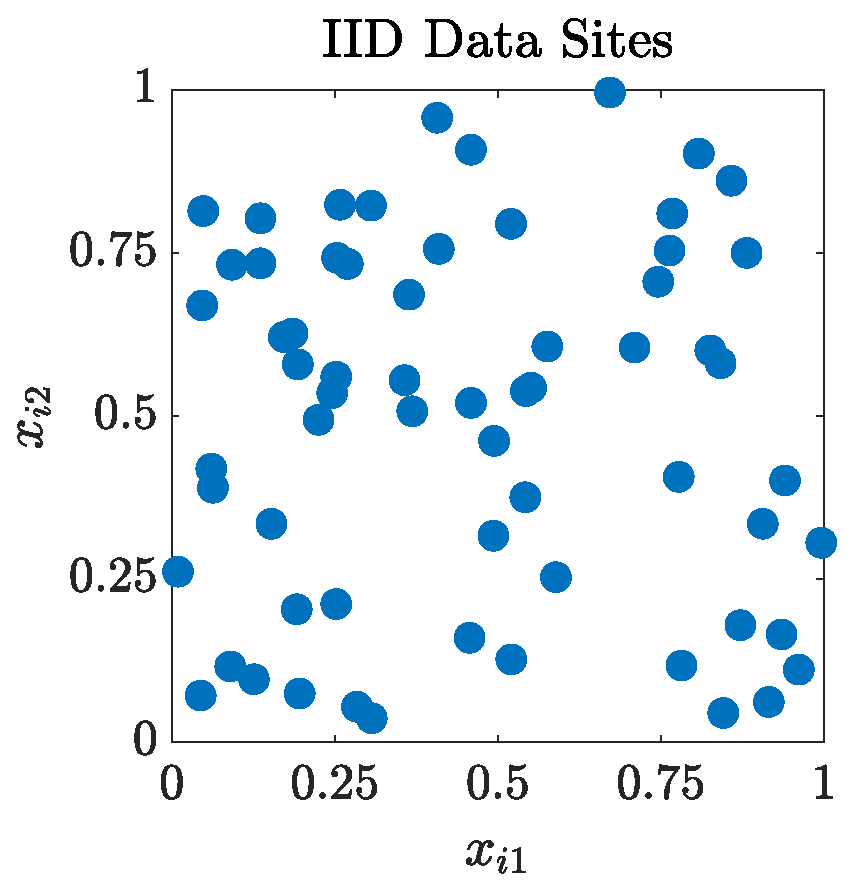
\includegraphics[width = 0.31\textwidth]{ProgramsImages/IIDPoints.eps} \quad
	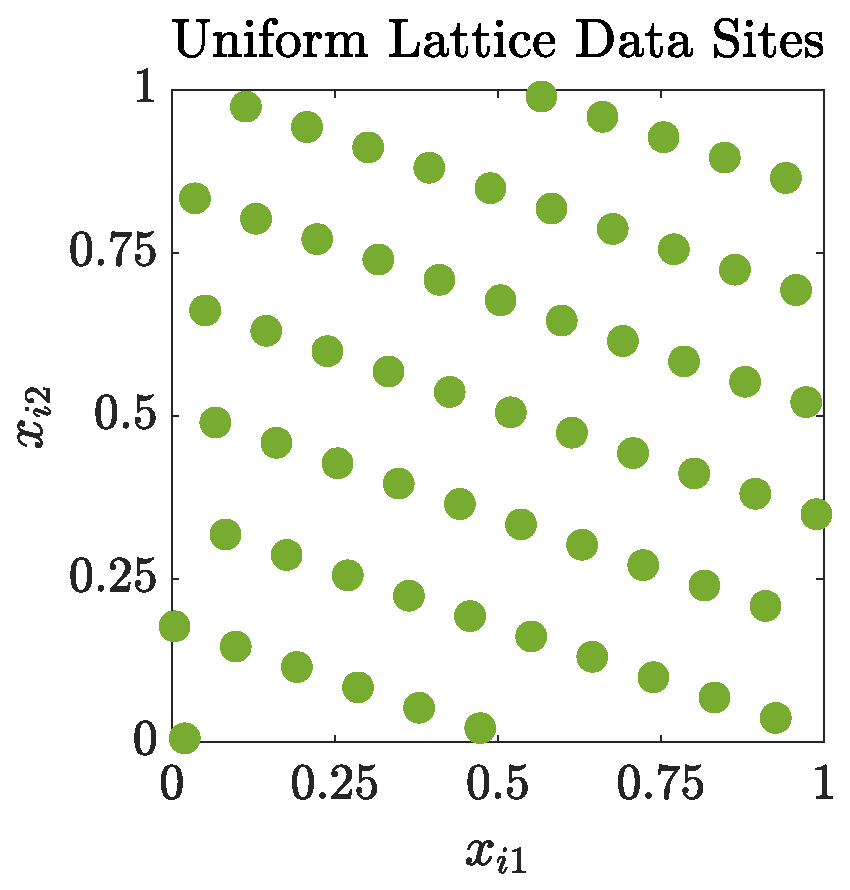
\includegraphics[width = 0.31\textwidth]{ProgramsImages/ShiftedLatticePoints.eps}  \quad
	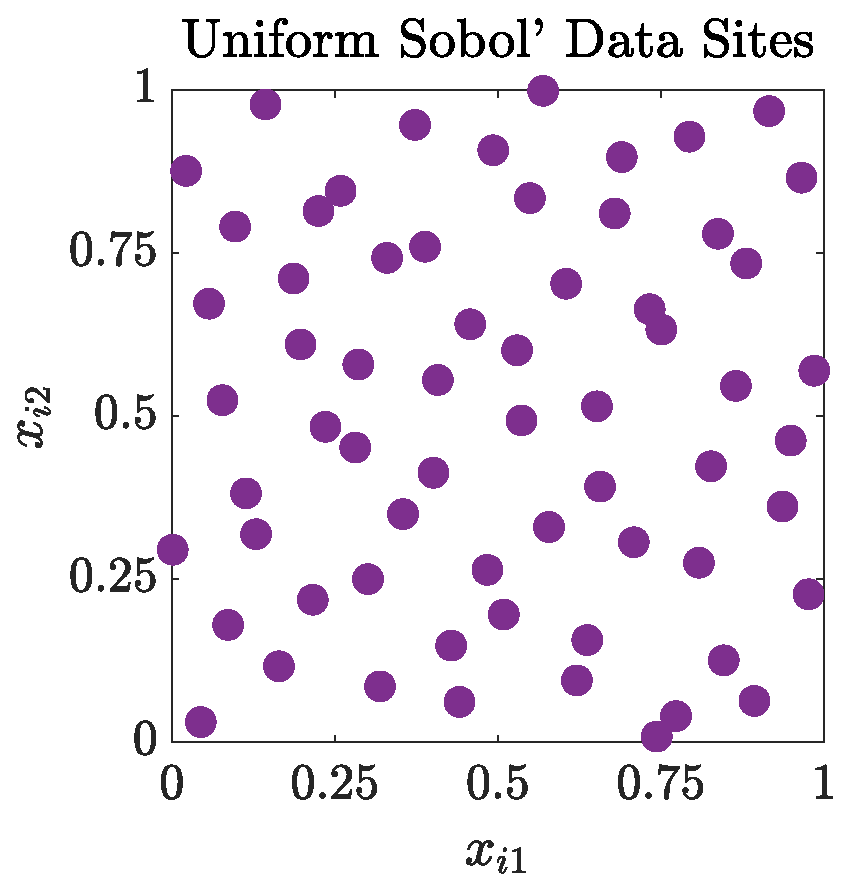
\includegraphics[width = 0.31\textwidth]{ProgramsImages/SSobolPoints.eps} 
	
	\caption{IID nodes contrasted with nodes used for QMC cubature.\label{PtsFig}}
\end{figure}

For the \QMC sampling considered here, $n$ is 
commonly a power of two.  The well-known theoretical error bound for 
\QMC cubature can be expressed in terms of some of the Fourier coefficients of the 
integrand \cite{DicEtal14a, DicPil10a, HicJim16a,JimHic16a, Nie92, SloJoe94}:
\begin{gather}
\nonumber
f(\bx) = \sum_{\bk \in \bbK} \hf(\bk) \phi_{\bk} (\bx),  \qquad \text{where } \hf(\bk) := \int_{[0,1]^d} 
f(\bx) \, \overline{\phi}_{\bk}(\bx) \quad \forall \bk \in \bbK, \\
\label{multiInt} \APP(f,n) = \frac 1n \sum_{i=1}^{n} f(\bx_i), \qquad
\abs{\SOL(f) - \APP(f,n)} \le \sum_{\bk \in P^\perp_n \setminus\{\bzero\}} \abs{\hf(\bk)} \\
\nonumber
\text{Dual set: }P_n^\perp : = \{\bk \in \bbK \, \vert \, \phi_{\bk}(\bx_i) = \phi_{\bk}(\bx_1) \text{ for } 
i=1, \ldots, n \}.
\end{gather}
For lattice nodes, $\bbK = \integers^d$ and the $\phi_{\bk}$ are complex exponentials.  For digital sequence nodes,  $\bbK = \natzero^d$ and the $\phi_{\bk}$ are Walsh functions.

FJH and LlAJR in \cite{HicJim16a,JimHic16a} defined a cone integrands, $\cc$, 
whose Fourier coefficients decay steadily, but  not necessarily monotonically.  The definition is technical, but Fig.\ \ref{GoodBadWalshFig} 
illustrates two functions and their Fourier 
(Walsh) coefficients, one inside the cone and one outside.  Here and in the error bound below, $\{\bk(\kappa)\}_{\kappa = 1}^\infty$ 
denotes an ordering of the $d$-dimensional wavenumbers in $\bbK$.

\begin{figure}[h]
	\centering
	\includegraphics[width = 0.23\textwidth] 
	{ProgramsImages/FunctionWalshFourierCoeffDecay.eps} \ \ 
	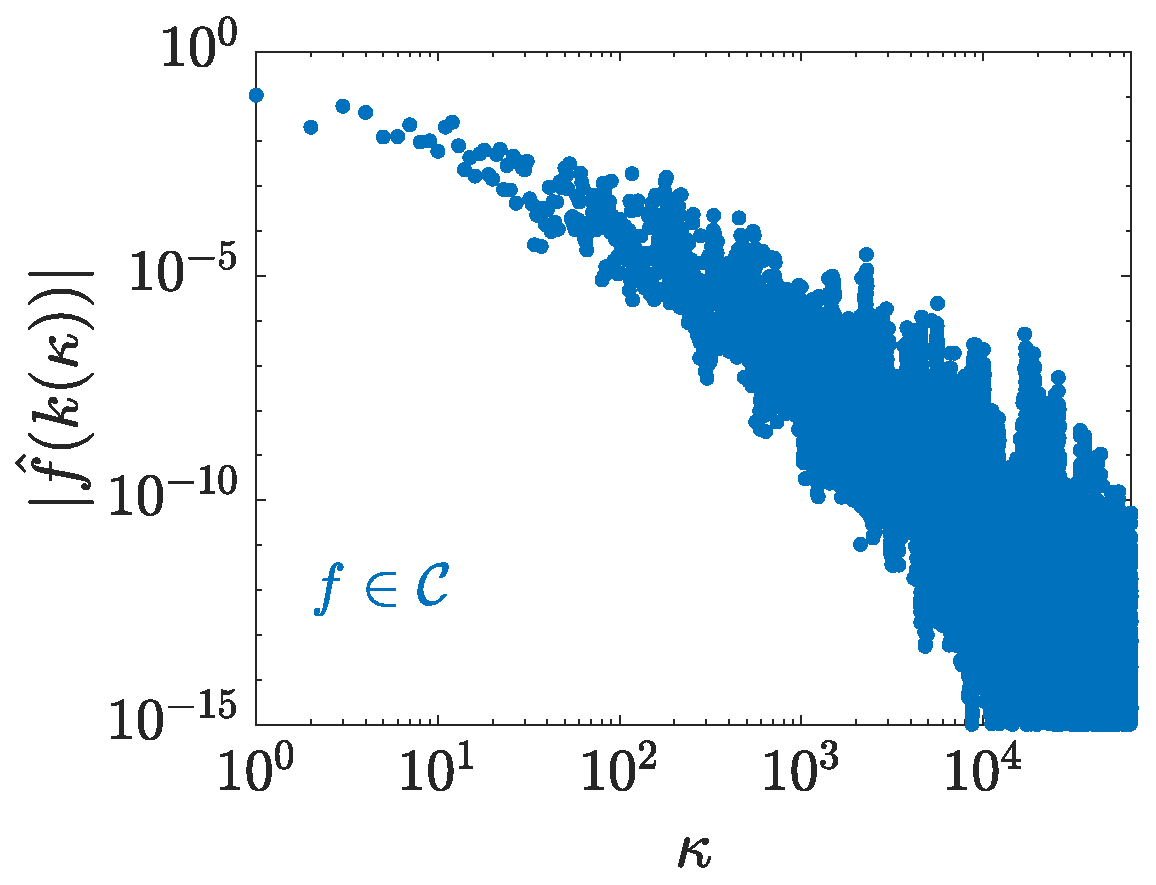
\includegraphics[width = 0.23\textwidth] 
	{ProgramsImages/WalshFourierCoeffDecay128.eps} \ \ 
	\includegraphics[width = 0.23\textwidth] 
	{ProgramsImages/FilteredFunctionWalshFourierCoeffDecay.eps} \ \ 
	\includegraphics[width = 0.23\textwidth] 
	{ProgramsImages/WalshFourierCoeffDecayFilter.eps}
	\caption{A function inside $\cc$ and another with high frequency noise outside $\cc$
		%and their Fourier coefficients 
	\label{GoodBadWalshFig}}
\end{figure}

This definition  of $\cc$ allowed us to derive a data-driven bound on the cubature error above in \eqref{multiInt} in terms of the \emph{discrete} Fourier coefficients: 
\begin{equation*}
\ERR(\dataN,n) = \fC(n) \sum_{\kappa = n/(2n_1) + 1}^{n/n_1} \abs{\tf_n(\bk(\kappa))}, \qquad \text{where } \tf_n(\bk)  = \frac{1}n \sum_{i=1}^{n} f(\bx_i) \overline{\phi}_{\bk}(\bx_i).
\end{equation*}
Here $\fC(n)$ is an inflation factor.  The data driven error bound depends on moderate-sized wavenumbers because they best emulate the error---which comes from large wavenumbers---but their discrete Fourier coefficients are not contaminated by aliasing. This data-driven error bound is used to construct guaranteed adaptive \QMC cubature 
algorithms: $n$ is increased by doubling until $\ERR(\dataN,n^*) \le \varepsilon$.  Then choosing 
$\ALG(f,\varepsilon) = \APP(f,n^*)$ satisfies 
\eqref{AlgErr}.  As in the cases of the univariate algorithms in Sect.\ \ref{sec:localadpat}, necessary conditions for $f$ to lie in $\calc$ arise from the cone definition.  Moreover, this algorithm automatically senses the speed at which the Fourier coefficients and converges accordingly; it is smoothness adaptable.

Using a fast transform to compute the discrete Fourier coefficients, the total cost is $\Order\bigl(\$_d(f)n^* + n^* \log(n^*)\bigr)$.  So, the cost of manipulating the function data is not much worse than the computational cost of collecting the function data, a concern raised in Sect.\ \ref{sec:CompEff}.

FJH, LlAJR, and DL generalized the adaptive \QMC rules to accommodate control variates \cite{HicEtal17a}.  We also extended adaptive cubatures to a more general error criterion.  Bayesian inference \cite{GelEtal13} and computing Sobol' indices \cite{Sal02a} involve a function of \emph{more than one} integral. We vectorized the solution operator, $\SOL : \calf^p \to \reals^p$, defined the answer as some function of this vector of integrals, $\Ans: \reals^p \to \reals$, allowed a relative error tolerance, $\reltol$, and constructed an $\ALG$ satisfying
\begin{multline}
\label{generrorcrit} \tag{G-ALG-CRIT}
\abs{\Ans(\SOL(\vf)) - \ALG(\vf,\varepsilon, \reltol) } \le \max(\varepsilon, \reltol \abs{\Ans(\SOL(\vf))} ) \\
\forall \vf \in \cc^p, \ \varepsilon > 0, \ 0 < \reltol < 1 .
\end{multline}
JL derived a similar generalization for an adaptive trapezoidal rule \cite{Liu17a}.


%%%%%%%%%%%%%%%%%%%%%%%%%%%%%%%%%%%%%%%%%%%%%%%%%%%%
\subsubsection{Adaptive Bayesian Cubature}  \label{sec:Bayes} 
%%%%%%%%%%%%%%%%%%%%%%%%%%%%%%%%%%%%%%%%%%%%%%%%%%%%
The research above assumes a deterministic integrand, but recent research by FJH and JR assumes that the integrand is an instance of a Gaussian process with constant mean $m$, and covariance kernel, $C:[0,1]^d \times [0,1]^d \to \reals$, i.e., 
$f \sim \GP (m,C)$.  This \href{http://www.probabilistic-numerics.org}{probabilistic numerics} approach dates back at least thirty years \cite{Dia88a, OHa91a, RasGha03a, Rit00a} and has generated recent interest. One constructs a credible interval in the Bayesian sense, $\Prob\bigl[\abs{\SOL(f) 
- \APP(f,n)} \le \ErrN \bigr] = 99\%$, where $\APP(f,n)$ is the posterior mean.  By increasing $n$ until the width of the credible interval is no greater than the error tolerance, one has an adaptive Bayesian cubature.  The hyper-parameters, $m$ and the parameters defining the covariance kernel, $C$, may be treated by empirical Bayes (maximum likelihood estimation), full Bayes, and/or cross-validation \cite{RatHic19a}.  Although similar computations can done assuming $C$ to be a reproducing kernel for a Hilbert space, the Gaussian process approach facilitates data-driven error bounds.

A longstanding drawback of Bayesian cubature has been the computational cost of operations
involving the Gram matrix $\mC = \bigl(C(\bx_i,\bx_j)\bigr)_{i,j=1}^n$, which is ordinarily
$\Order(n^3)$.  Attempts to overcome this cost include \cite{AniCheSte16a, ParEtal17a}.  FJH and JR chose shift-invariant covariance kernels, which matched the lattice nodes used for sampling the integrand \cite{RatHic19a}. This yields Gram matrices $\mC$ for which the necessary vector-matrix operations can be accomplished by fast transforms with computational cost $\Order(n 
\log(n))$, making Bayesian cubature practical.  We also found a way to avoid the round-off error that often plagues these Gaussian process methods for large $n$.

The following table shows the performance of our adaptive cubatures in approximating the integral corresponding to the price of Asian arithmetic mean call option where the price is $\$13.12$ and $d=12$.  The cubatures were run under different scramblings of the nodes.
\[
\begin{array}{cccccr@{.}l}
    \text{Error} & & \text{Median} & & \text{Worst }10\% & \multicolumn{2}{c}{\text{Worst }10\%}\\
    \text{Tolerance} & \text{Method} & \text{Error} & \text{Success} & n & \multicolumn{2}{c}{\text{Time (sec)}} \\
    \toprule
     1\text{E}-2& \text{IID Monte Carlo \cite{HicEtal14a}} & 2\text{E}-3 & 100\% & 6.1\text{E}7 & 33\\
     1\text{E}-2&  \text{Lattice Nodes \cite{JimHic16a}} & 1\text{E}-3 & 100\% & 1.6\text{E}4 & 0&041\\
     1\text{E}-2& \text{Sobol' Nodes \cite{HicJim16a}} & 1\text{E}-3 & 100\% & 1.6\text{E}4 & 0&040\\
     1\text{E}-2&  \text{Sobol' Nodes w/ Control Variates \cite{HicEtal18a}} & 2\text{E}-3 & 100\% & 4.1\text{E}3 & 0&019\\
     1\text{E}-2& \text{Bayesian w/ Lattice Nodes \cite{RatHic19a}} & 2\text{E}-3 & 99\% & 1.6\text{E}4 & 0&051\\
\end{array}
\]

%%%%%%%%%%%%%%%%%%%%%%%%%%%%%%%%%%%%%%%%%%%%%%%%%%%%
\subsubsection{Multivariate Function Approximation} \label{sec:PrevFunAppx}
%%%%%%%%%%%%%%%%%%%%%%%%%%%%%%%%%%%%%%%%%%%%%%%%%%%%

GEF has led the effort in accurate, well-conditioned function approximation and solution of 
differential equations using reproducing kernel Hilbert space methods.  Much of his effort has been 
developing truncated Hilbert-Schmidt decomposition of the reproducing kernels using appropriate 
eigenfunctions.  For example, an expansion of the squared exponential (Gaussian) kernel using 
Chebyshev polynomials instead of Hermite polynomials has been used for the numerical solution of 
nonlinear unsteady 
convection-diffusion-reaction equations.  GEF and his collaborators extended
decompositions of the Matern kernels on the half line to the entire real line, the first such analytical 
derivations.

FJH, YD, and LlAJR investigated the solution of general linear operators, $\SOL$, when series coefficients are available \cite{DinHic20a}.  Suppose that 
\begin{subequations} \label{serForm}
\begin{gather}
    \calf := \left \{ \sum_{\bk \in \caln} \hf(\bk) u_{\bk} : \norm[\calf]{f} := \norm[r]{\left(\frac{\bigabs{\hf(\bk)}}{\lambda_{\bk}} \right)_{\bk \in \caln}} \right \},  \quad
    \calg : = \biggl \{ \sum_{\bk \in \caln} \hg(\bk) v_{\bk} : \norm[\calg]{g} := \bignorm[r']{\hg}\biggr \}, \\ 
    v_{\bk} = \SOL(u_{\bk}), \quad
     \lambda_{\bk_1} \ge \lambda_{\bk_2} \ge \cdots, \qquad
      n_0 < n_1 < n_2 < \cdots, \quad r^{-1} + r'{}^{-1} = 1.
\end{gather}

\end{subequations}
By assuming a steady decay of the series coefficients, ordered according to the $\lambda_{\bk}$, and for the case $r=2$, we constructed an adaptive algorithm defined on a cone, $\cc \subset \calf$, and based on sampling \emph{Fourier coefficients}, not function values.  This algorithm is essentially optimal.


%%%%%%%%%%%%%%%%%%%%%%%%%%%%%%%%%%%%%%%%%%%%%%%%%%%%
\subsection{Broader Impacts from Previous NSF Funding} \label{prevBIsect}
%%%%%%%%%%%%%%%%%%%%%%%%%%%%%%%%%%%%%%%%%%%%%%%%%%%%

\emph{Publications, Conference Participation, and Conference Organization.} Publications by GEF, FJH,  SCTC, students, and collaborators are listed at the beginning of this section.  We have spoken at many applied mathematics, statistics, 
and computational science conferences and given colloquium/seminar talks to mathematics and 
statistics departments.  Here are highlights.  FJH, SCTC, LJ, and LlAJR published  an 
encyclopedia entry on adaptive Monte Carlo \cite{HicEtal18a}.  FJH co-organized the 
\href{http://cos.iit.edu/2016-spring-research-conference/}{2016 Spring Research 
Conference}, a long-running annual industrial statistics conference.   FJH gave an invited tutorial 
at the \href{http://mcqmc2016.stanford.edu}{MCQMC 2016} 
\cite{Hic17a}, a biennial conference for which he serves on the steering committee.  FJH 
was a program leader for the SAMSI 2017--18 
\href{https://www.samsi.info/programs-and-activities/year-long-research-programs/2017-18-program-quasi-monte-carlo-high-dimensional-sampling-methods-applied-mathematics-qmc/
}{\QMC Program (\hypertarget{SAMSIlink}{SAMSI-QMC})}.   He  gave an invited tutorial 
	at the Opening Workshop, and led one of 
	the working groups.  FJH received the 2016 Joseph F.\ Traub 
	Prize for Achievement in Information-Based Complexity.
	
	
FJH's leadership in the MCQMC conferences  and \SAMSIQMC brought \QMC to other areas of potential application.  One concrete example, is the 
	collaboration between FJH, LlAJR and French collaborators working in uncertainty quantification \cite{GilEtal16a, GilJim16b}.  Another example, is the collaboration of LlAJR with
	high energy physicists at Fermilab, in the Chicago suburbs, using \QMC to speed 
	up their calculations.
	
\emph{\GAIL Software.} The results of this research have been implemented in 
\GAIL, our open source \MATLAB library hosted on
\href{http://gailgithub.github.io/GAIL_Dev/} {Github}. This software 
has been implemented with input parsing, input validation, unit tests, inline documentation, and 
demonstrations.  \GAIL makes it easier for practitioners to try our new adaptive algorithms.  SCTC has been key in this effort.  
%With the help of students, we are starting to port GAIL to Python and \Rlang.

\emph{Boosting the STEM Workforce.} GEF, FJH, and SCTC have mentored a number of 
research students associated with this project.  The main ones are mentioned at the beginning of 
this section.  Female students mentored include YD, LJ, JL, XT, and Xiaoyang Zhao (MS 2017).   GEF, FJH,  and SCTC have mentored many undergraduate students including more than a dozen 
Brazilian Science Mobility Program students in the summers of 2015 and 2016, Noah Grudowski (BS student IIT), Cu Hauw Hung (BS Biola U, now MS student at UCLA), Tanner Johnson (BS U Minnesota, now MS student at U British Columbia), Yueyi Li (female, BS Macalester U, now MS student at Johns Hopkins), Tianpei Qian (BS NUS, now MS student at Stanford), Alexsei Sorokin (BS student IIT), Paul Wolfert (BS student Colorado Schoo of Mines), and 
Tianci Zhu (female, now MS student at NYU).  We have also had a few high school students join us. As part of our team, all of
these students have learned how to conduct theoretical and/or practical computational mathematics research.

FJH has taught a course on Monte Carlo methods each fall.  For the past several years students 
have been introduced to \GAIL and used it in their coursework.  \GAIL has been used to teach how 
to know how large $n$ must be for an \IIDMC or \QMC simulation to reach the desired accuracy 
requirement.  A number of student class projects have been devoted to improving \GAIL.

In recognition of his research leadership, FJH was appointed the director of Illinois Tech's new Center for Interdisciplinary 
Scientific Computation in 2017.  In this position he fostered collaborative scientific computation 
research across departments by hosting matchmaking seminars and sponsoring a seed grant 
competition. In 2018, FJH was appointed Vice Provost for Research.




%%%%%%%%%%%%%%%%%%%%%%%%%%%%%%%%%%%%%%%%%%%%%%%%%%%%
\section{Intellectual Merit of the Proposed Research} \label{sec:Proposed}
%%%%%%%%%%%%%%%%%%%%%%%%%%%%%%%%%%%%%%%%%%%%%%%%%%%%


%%%%%%%%%%%%%%%%%%%%%%%%%%%%%%%%%%%%%%%%%%%%%%%%%%%%
\subsection{Adaptive Algorithms for Multivariate Integration}\label{SectMultiInt}
%%%%%%%%%%%%%%%%%%%%%%%%%%%%%%%%%%%%%%%%%%%%%%%%%%%%

%%%%%%%%%%%%%%%%%%%%%%%%%%%%%%%%%%%%%%%%%%%%%%%%%%%%
\subsubsection{Fast Bayesian Cubature Using Higher Order Digital Nets}  \label{sec:NewBayes}
%%%%%%%%%%%%%%%%%%%%%%%%%%%%%%%%%%%%%%%%%%%%%%%%%%%%

The fast Bayesian cubature  described in Sect.\ \ref{sec:Bayes} \cite{RatHic19a} has been fully implemented for lattice node \QMC sampling, but not yet for the digital sequence node \QMC sampling.  Although this should work in principle, we are particularly interested in employing higher order nets with matching kernels based on Walsh functions to obtain higher order accuracy.  As is the case for lattices, the kernels need to match the nodes to ensure that the algorithm is fast enough (Goal \ref{GoalThree}).

To justify the Bayesian cubature assumption that $f$ is a Gaussian process, we have plotted normal probability plots of suitably scaled sample function values.  However, the distribution does not follow a Gaussian.  Student $t$-processes have been proposed \cite{ShaWilGha14a}, and we will explore non-Gaussian processes in the hope that the Bayesian approach can find a more solid footing.

There have not yet been tractability studies (see Sect.\ \ref{sec:CompEff}), which we intend to do. To implement covariance kernels that yield tractable problems might require a finer structure in our covariance kernels, namely, a weight for each coordinate.  This will require us to implement a more  sophisticated optimization of the kernel hyper-parameters than we have done already.  This is also needed to ensure that our algorithm can capture and take advantage of different degrees of smoothness.

\subsubsection{Generalized Error Criterion for IID Monte Carlo.}  LJ developed an adaptive \IIDMC algorithm satisfying a hybrid error criterion encompassing both absolute and relative error in her PhD thesis \cite{Jia16a}.  However, her error criterion is not as general as \eqref{generrorcrit}.  We will generalize LJ's work to 
cover this case (Goal \ref{GoalFour}).  Recently \cite{KunEtal19a} use the median of means method to derive an adaptive \IIDMC cubature satisfying \eqref{AlgErr}.  We think that there method might be more flexible than  LJ's, which relied on Berry-Eseen inequalities.  We will explore that route.


%%%%%%%%%%%%%%%%%%%%%%%%%%%%%%%%%%%%%%%%%%%%%%%%%%%%
\subsubsection{Integration with Unbounded Dimension} \label{sec:InfDim}
%%%%%%%%%%%%%%%%%%%%%%%%%%%%%%%%%%%%%%%%%%%%%%%%%%%%

Taking the expected value of a function of the solution to a stochastic differential equation(SDE)---as is required in finance calculations---takes the form of an infinite dimensional integral, namely,
\[
\SOL(f) = \lim_{d \to \infty} \SOL_d(f_d), \quad \SOL_d(f_d):= \int_{\reals^d} f_d(\bx) \, \prod_{r=1}^{d} \varrho(x_r) \, \dif \bx, 
\]
where $f_d$ is an  approximation to $f$ that depends only on the first $d$ variables, and $\varrho$ 
is a univariate probability density function.  In the application described above $d$ represents the number of time steps in the discretized SDE.

Approximating $\SOL(f)$ by $\SOL_{d_L}(f_{d_L})$ for some large $d_L$ incurs the expensive, typically $\Order(d_L)$ cost per function value.  Two alternative methods for approximating $S(f)$ are the multi-level method (MLM) \cite{Gil15a} and the  multivariate 
decomposition method (MDM) \cite{Was13b}.  (The MLM for cubature is inspired by the MLM 
for solving partial differential equations, but is quite different.) The function $f$
is decomposed into pieces that only depend on the a subset of the coordinates (see 
\cite{WanHic00b} for example):  
\begin{equation*}
f(\bx) = \sum_{\fu \subset \naturals, \abs{\fu} < \infty} f_{\fu}(\bx) = \sum_{\ell 
=1}^\infty [f_{d_\ell}(\bx) - f_{d_{\ell-1}}(\bx)], \qquad  f_d:= \sum_{\fu \subseteq \{1, 
\ldots, d\}} f_\fu, \quad f_0:= 0.
\end{equation*}
Here $\abs{\fu}$ denotes the cardinality of the set $\fu$.  Each $f_{\fu}$ depends only 
on the coordinates with indices in $\fu$.  If $\APP_{d}$ represents a cubature 
using on the $d$-dimensional domain, then the MLM and MDM cubatures 
for approximating $\SOL(f)$ are 
\begin{gather*}
\APP^{\textup{MLM}}_{L,\bd}(f,\bn) = \sum_{\ell=1}^L \APP_{d_\ell}(f_{d_\ell} - f_{d_{\ell-1}},n_\ell), \qquad 
\bn = (n_\ell)_{\ell = 1}^L, \quad \bd = (d_\ell)_{\ell = 1}^L, \\
\APP^{\textup{MDM}}_{\fU,\bd}(f,\bn) = \sum_{\fu \in \fU} \APP_{\abs{\fu}}(f_{u},n_{\fu}), \qquad 
\bn = (n_\fu)_{\fu \in \fU}, \quad \bd = (d_\fu)_{\fu \in \fU}, \quad  \\
\cost(f,\APP^{\textup{MLM}}_{L,\bd},\bn) = \Order\left (\sum_{\ell=1}^L d_\ell 
n_\ell \right), \qquad 
\cost(f,A^{\textup{MDM}}_{\fU,\bd},\bn) = \Order\left (\sum_{\fu \in \fU} d_\fu 
n_\fu\right)
\end{gather*}
The advantage of these methods is that typically large dimensions, $d_\ell$ or $d_{\fu}$, require only small sample sizes, $n_\ell$ or $n_\fu$.  This keeps the total cost down and helps us meet Goal \ref{GoalThree}.

Existing stopping criteria for MLMs and MDMs are based on heuristics.  We will use the lessons learned in our previous research, summarized in  Sects.\ \ref{sec:QMC} and \ref{sec:Bayes} to derive rigorous stopping criteria for MLMs and MDMs. These stopping criteria will include not only the choice of sample sizes but also the suitable choice of data-driven decompositions of the infinite dimensional integrand.  FJH's familiarity with the MLM \cite{HicMGRitNiu09a, NiuHic09a, NiuHic09b} will facilitate this task.

%%%%%%%%%%%%%%%%%%%%%%%%%%%%%%%%%%%%%%%%%%%%%%%%%%%%
\subsection{Adaptive Multivariate Function Approximation}
%%%%%%%%%%%%%%%%%%%%%%%%%%%%%%%%%%%%%%%%%%%%%%%%%%%%

%%%%%%%%%%%%%%%%%%%%%%%%%%%%%%%%%%%%%%%%%%%%%%%%%%%%
\subsubsection{Tractability} \label{sec:tract}
%%%%%%%%%%%%%%%%%%%%%%%%%%%%%%%%%%%%%%%%%%%%%%%%%%%%

We will study the tractability of the general linear problems studied by YD, FJH, and LLAJR in \cite{DinHic20a} (see Sect.\ \ref{sec:PrevFunAppx}).  Tensor product spaces will be assumed.  FJH has contributed to the tractability literature for balls of input functions
\cite{FasHicWoz12b,WanHic00b,HicWoz00b,HicSloWas03c,HicSloWas03b,HicSloWas03a,HicSloWas03e,HicWasWoz06a,YueHic04a,YueHic05a,ZhoHic15a}.  This will help us complete this study for cones of input functions (Goal \ref{GoalThree}).

The tractability literature tends to use the same techniques applied separately to many different cases:  strong tractability, polynomial tractability, quasi-polynomial tractability, weak tractability, algebraic tractability, and exponential tractability.  We aim to develop a more unified treatment that would reduce the number of proofs required. Not only would this apply to the case of balls of input functions but also the case of cones of input functions, which particularly interests us.


%%%%%%%%%%%%%%%%%%%%%%%%%%%%%%%%%%%%%%%%%%%%%%%%%%%%
\subsubsection{Function approximation using matching kernels and nodes}
%%%%%%%%%%%%%%%%%%%%%%%%%%%%%%%%%%%%%%%%%%%%%%%%%%%%

The Bayesian framework may also be used for function approximation as well as cubature.  This approach is known as kriging or Gaussian process modeling in the statistics literature \cite{RasWil06a,Ste99} and is known as meshfree/radial basis function 
approximation in the numerical analysis literature \cite{Fas07a,FasMcC15a,Wen05a}.  We will employ the \QMC node sequences with their well-matched kernels for adaptive multivariate function 
approximation, as we have done and plan to do for cubature (Sects.\ \ref{sec:Bayes} and \ref{sec:NewBayes}).  Because we are using matching kernels, we will reduce the matrix operations costing that typically cost $\Order(n^3)$ to only $\Order(n \log(n))$.  We will also explore some of the designer kernels developed by GEF in our previous NSF-funded  project (Sect.\ \ref{sec:PrevFunAppx}).  Because the theoretical error bounds \eqref{errorBd} for function approximation using \QMC node sequences are under-developed, there is much to be done.

%%%%%%%%%%%%%%%%%%%%%%%%%%%%%%%%%%%%%%%%%%%%%%%%%%%%
\subsubsection{Problems with Expensive Function Values} 
\label{sec:Expensive}
%%%%%%%%%%%%%%%%%%%%%%%%%%%%%%%%%%%%%%%%%%%%%%%%%%%%

When the cost of one $f(\bx)$ takes hours or days, as in a climate model or simulating the performance of a huge financial portfolio, it helps to have surrogates models: approximations to $f$ that are cheap to evaluate.  For these situations---mentioned in Sect.\ \ref{sec:CompEff}---the cost of manipulating $n^*$ data, say $\Order(n^{*p})$ is unimportant compared to the cost of acquiring $n^*$ data, $\$_d(f)n*$.  Perhaps, only $\Order(d)$ function values can be afforded.  This problem has been discussed by a \SAMSIQMC working group led by FJH over the last year, and we have some preliminary thoughts.  

Consider the situation in \eqref{serForm} with $r = \infty$.  The function approximation problem means $\SOL(f) = f$ and $v_{\bk} = \SOL(u_{\bk}) = u_{\bk}$.  The optimal fixed sample size approximation and its error bound, assuming that we can sample Fourier coefficients, is 
\begin{gather*}
    \APP(f,n) = \sum_{i=1}^n \hf(\bk_i) u_{\bk_i}, \qquad
    \norm[\calg]{\SOL(f) - \APP(f,n)} %= \bignorm[1]{\bigl(\hf(\bk_i)\bigr)_{i=n+1}^\infty } 
    \le \norm[1] {\bigl(\lambda_{\bk_i}\bigr)_{i=n+1}^\infty } \norm[\calf]{f}.
\end{gather*}
We may then use the model Algorithm \ref{ConeAlg} to obtain an adaptive algorithm.  

One important question is how to choose the $\lambda_{\bk}$.  We want to infer them.  Appropriating the principles of effect sparsity, effect hierarchy, and effect heredity from the statistical experimental design literature \cite{WuHam00}, and borrowing the concept of coordinate weights from the tractability literature \cite{DicEtal14a}, our \SAMSIQMC working group proposed tensor product spaces with the following weights:
\[
\bk \in \natzero^d, \qquad u_{\bk} = \phi_{k_1} \cdots \phi_{k_d}, \qquad \lambda_{\bk} = \prod_{\substack{\ell = 1 \\ k_{\ell} > 0 }}^d \gamma_{\ell}s_{k_\ell} 
\qquad \begin{cases} \phi_k = \text{a polynomial of degree }k, \\
\gamma_{\ell} = \text{coordinate importance}, \\
s_{k} = \text{smoothness degree}.
\end{cases}
\]

As proof of concept of this approach, we used a screening sample of size $\Order(d)$ that  explored the dependence in each coordinate direction, inferring the coordinate importances and the smoothness degrees, and then followed the procedure of Algorithm \ref{ConeAlg}.  Instead of assuming that we knew the Fourier coefficients, we approximated them by polynomial interpolation.  We chose a polynomial basis for which $\norm[\infty]{\phi_k} = 1$, so that $\norm[\infty]{f - \ALG(f,\varepsilon)} \le \norm[\calg]{f - \ALG(f,\varepsilon)}$.  We tried this procedure on a test function of \cite{ChenSan10a} from \cite{VirLib17a} for a variety of $\varepsilon$.  The results are in Fig.\ \ref{fig:ChengSand}.

\begin{figure}
    \centering
    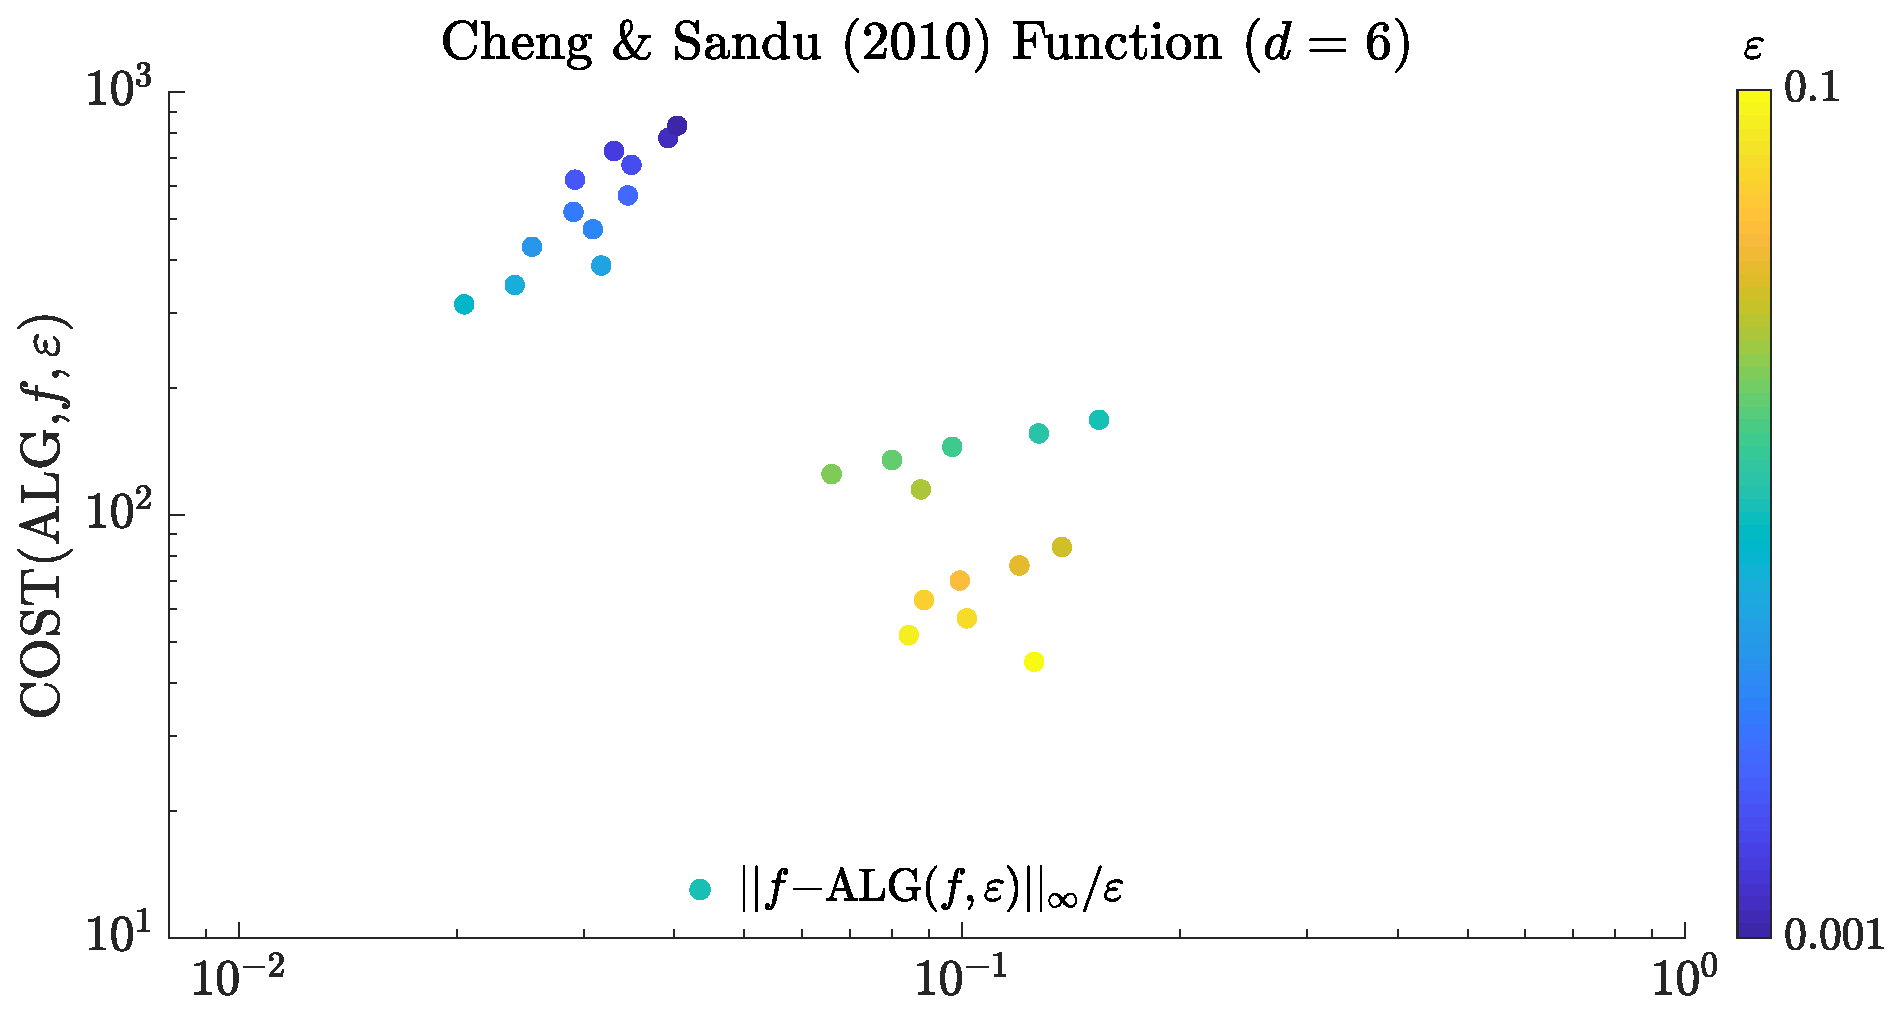
\includegraphics[height = 5cm]{ProgramsImages/sim_eval_results_chsan10_d6_sflg1ErrN.eps}
    \caption{Pilot function approximation algorithm for $\varepsilon$ ranging from $0.001$ to $0.1$}
    \label{fig:ChengSand}
\end{figure}

While this preliminary study is encouraging, there is  still much to do.  We need to establish theoretically for which cones of functions, we can infer the $\gamma_{\ell}$ and $s_k$ using a screening sample of function values and meet the error tolerance with a sample size approximately $\Order(d)$.  In this kind of problem, we are not concerned about the cost of polynomial interpolation because this method is intended for problems where the cost of data acquisition dominates.

%%%%%%%%%%%%%%%%%%%%%%%%%%%%%%%%%%%%%%%%%%%%%%%%%%%%
\subsection{Higher Order Adaptive Algorithms for Univariate Problems}\label{SectUniProb}
%%%%%%%%%%%%%%%%%%%%%%%%%%%%%%%%%%%%%%%%%%%%%%%%%%%%

Although the proposed research focuses primarily on algorithms for multivariate problems, we will devote some effort to better algorithms for univariate problems.  Now that YZ has established an adaptive Simpson's rule with a theoretically justified stopping criterion, we are better prepared to derive a theoretically justified stopping criterion for \MATLAB's 
\texttt{integral.m}, which will allow it to succeed for fluky functions like the one depicted in Fig.\ \ref{quadfailfig}b).  Instead of comparing two different quadratures that share the same nodes, we will approximate the norm of the derivative that controls the error of the Gauss quadrature.

\Chebfun is popular, but it too is lacking a rigorous foundation.  We will define a cone of functions $\cc$, for which \Chebfun must give the correct answer.  This will be done in a similar manner as for \QMC quadrature in Sect.\ \ref{sec:QMC}.  The cone $\cc$ will consist of functions 
whose Chebyshev series does not decay erratically for terms with polynomial degree greater than 
some minimum value.  Spiky functions will be excluded from $\cc$.  As a side note, \Chebfun recently increased their default initial sample size to be more robust against spikes.

\MATLAB's \texttt{fminbnd} and similar algorithms are local optimizers, whereas our algorithm described in Sect.\ \ref{sec:localadpat} is a guaranteed global optimizer, and thus a viable alternative.  We would like to improve its convergence rate by performing quadratic search and place it commonly used software libraries.

%%%%%%%%%%%%%%%%%%%%%%%%%%%%%%%%%%%%%%%%%%%%%%%%%%%%
\section{Broader Impacts of the Proposed Research}\label{SectBroad}
%%%%%%%%%%%%%%%%%%%%%%%%%%%%%%%%%%%%%%%%%%%%%%%%%%%%


%%%%%%%%%%%%%%%%%%%%%%%%%%%%%%%%%%%%%%%%%%%%%%%%%%%%
\subsection{Contributions to Training, Mentoring and Other Human Resource Developments}
%%%%%%%%%%%%%%%%%%%%%%%%%%%%%%%%%%%%%%%%%%%%%%%%%%%%
FJH leads a weekly research group meeting comprised of long-term and short-term student 
collaborators, visitors, the curious, and special guests.  Ongoing work in early or polished stages is shared.  Papers of other authors are presented.  Mentoring takes place during these meetings as well as individually.

\emph{Providing Research Experiences for Undergraduate and High School Students.} Students 
should be introduced to research before graduate school so that they can learn how to 
discover the unknown, something that is not necessarily taught in the classroom. We request funds 
to 
support two summer undergraduate students per year.  Our small summer research program has established some visibility 
and is prompting inquiries from prospective participants well before we 
even announce our latest 
offerings. As in the past, we expect the NSF funds will serve as a catalyst for funds to 
support additional summer students. In choosing summer students we will make a deliberate effort to 
build 
a diverse research environment by targeting female and underrepresented minority students as well 
as students from less research-focused institutions (see Sect.~\ref{prevBIsect}). We will also 
welcome well-prepared high school students to join our research group.

\emph{Preparing Students for Academic Careers.} Mentoring is a multi-faceted and 
potentially long-term process continuing even after the mentee has moved on from Illinois Tech.  
Our PhD students gain experience both research and mentoring the younger students in our 
research group.  We 
continue contact with many of our former students.  In particular we continue to 
collaborate with YD and Yiou Li (female).  We will continue to help our students prepare for 
academic careers and continue mentoring them after they leave Illinois Tech.

\emph{Preparing Students for Industry Careers.}
We also help current students land 
competitive jobs in the business world. Our training in the areas of computation and software 
development gives our students the needed edge in comparison to other mathematics 
graduates. For example, LlAJR and XZ are working in the financial services industry and  LJ is 
working in marketing analytics.  All of them are developing and testing quantitatively sophisticated 
and computationally intensive models.  LlAJR and LJ continue to collaborate with us on research.

\emph{Supervising Visitors.}
Both FJH and SCTC have strong connections to East Asia.  We have hosted several long-term 
self-funded visitors in the past and plan to do so in the future.

\emph{Giving Tutorials and Invited Lectures.}
We will continue providing lectures to students at various stages in their careers, ranging from high
school to graduate school. These encourage students to enter STEM and encourage STEM students 
to engage in research in general, and this research area in particular.


%%%%%%%%%%%%%%%%%%%%%%%%%%%%%%%%%%%%%%%%%%%%%%%%%%%%
\subsection{Contributions to Resources in Research, Education and the Broader Society} 
\label{BroaderTwoSec}
%%%%%%%%%%%%%%%%%%%%%%%%%%%%%%%%%%%%%%%%%%%%%%%%%%%%

The proposed research straddles mathematics, statistics, theoretical computer science, and 
application areas.  The two PIs have complementary strengths that facilitate this interdisciplinary research.  FJH 
has expertise in \QMC methods, kernel-based methods, information-based complexity 
theory, tractability, and experimental design. SCTC has expertise in computer science and applications.  Our 
expertise provides both an obligation and an opportunity to interact with a number of diverse 
communities. We envision the following contributions:

\emph{Disseminating Research}
The research supported by this grant will result in publications in peer-reviewed journals in applied
mathematics, computer science, statistics, and science/engineering. These 
journals will include both those that emphasize theory and those that emphasize applications.

\emph{Promoting Cones.} The idea of guaranteed, adaptive algorithms via cones of reasonable input 
functions has broad potential application.  We will continue to promote this idea among numerical analysts 
who 
develop new algorithms and analyze their computational costs, as well as among information-based 
complexity theorists who analyze the lower bounds on the complexity of numerical problems.  The recent work by Kunsch, Novak, and Rudolf \cite{KunEtal19a} shows that the idea of cones is catching on.

\emph{Bridging Applied Mathematics and Statistics.}
This project touches on topics that are of interest to the statistics community: kriging, Monte Carlo methods, probabilistic numerics, and design of experiments.  We have and will continue to engage the statistics community 
by speaking a their conferences and departmental colloquia.

\emph{Organizing and Presenting at Conferences.}
We and our students involved in this project will present our results at a variety of conferences and workshops.  These include: (i) specialized meetings focusing on approximation theory, complexity, 
experimental design, Monte Carlo methods, and probabilistic numerics; (ii) the national meetings of AMS, SIAM, and the 
statistical societies; and (iii) conferences devoted to application areas.  We are frequently invited to 
speak at such conferences, which will give our results a prominent hearing. We will also continue to 
organize specialized conferences or minisymposia within larger conferences.

\emph{Writing Survey Papers.}
FJH and SCTC will continue their practice of writing tutorial, survey, and encyclopedia articles.  These will make our findings accessible to a wider audience.

\iffalse
\emph{Refreshing Course Syllabi.}
MATH 565 (Monte Carlo Methods in Finance), taught every fall by FJH, has incorporated our new
results on guaranteed (quasi-)Monte Carlo multivariate integration. In the future it will include our 
new results on our guaranteed MLM and MDM (see Sect.\ \ref{SectMultiProb}).

As noted in Sect.\ \ref{TrapIllSect}, current texts propagate poor practices for 
adaptive quadrature.  We will urge numerical analysis textbook authors and educators to change the 
way that error estimation is taught based on our recent and proposed work.  These ideas will also 
enter our more traditional numerical analysis courses such as MATH 350 (Intro to Computational 
Math).  SCTC and FJH will continue to develop MATH 573 (Reliable Mathematical Software) as a 
valuable course for our own students and an example that we wish to propagate to other 
universities.
\fi

\emph{Creating Software and Collaborating with Software Developers.}
As the complexity of large scale numerical computations increase rapidly, mundane operations such as integration and function approximation are taken for granted. We must construct reliable adaptive algorithms for these problems so that there are no unwelcome surprises for the practitioner when she takes them for granted.

We will continue to develop \GAIL \citep{ChoEtal17b} (now up to version 2.2).  The \GAIL software 
will serve the wider community that relies on numerical approximation and integration algorithms.  It will 
also demonstrate how adaptive algorithms ought to be implemented, which we hope will inspire and 
inform those working on adaptive algorithms for other mathematical problems.  We will involve 
students in porting \GAIL to other platforms, such as Python, \Rlang, and \Julia.  

In the summer of 2018, we began engaging with other \QMC research groups about combining our software efforts.  These included the groups of Mike Giles (Oxford, Multi-Level Monte Carlo),  Frances Kuo (UNSW, \QMC generators, PDEs with random coefficients),  Dirk Nuyens (KU Leuven, \QMC generators, PDEs with random coefficients), and Christoph Schwab (ETH-Zurich, PDEs with random coefficients).  All of these groups have significant software development efforts, but our software libraries are not compatible with one another.  We have begun discussing a common framework for a shared community quasi-Monte Carlo software library, \QMCSoft.  If all groups would write their software to the specifications of this framework, then improvements and additions would immediately work with the other parts of the library.

We will collaborate with these other research groups to move our software to this common framework.  Given the difficulty in agreeing upon one language, this may be a multi-language effort.  We will seek resources outside this proposal to support this effort.  As the \QMC community embraces \QMCSoft, we expect our core of contributors to grow.  Scholars who develop new \QMC algorithms or use \QMC in applications will be encouraged to add them to \QMCSoft.  

We expect our new algorithms to be incorporated into widely used numerical packages, as was done for our algorithm in \cite{HonHic00a} by \MATLAB and \NAG.  We have already and will continue 
to discuss with software developers about good practices for adaptive algorithms.


\emph{New Applications of \QMC.}
The application of \QMC has focused on a few areas, such as financial modeling and computer 
graphics, but there is potential for much wider application.  LlAJR has collaborated with Fermilab implementing \QMC algorithms, and we plan to continue.    New applications of \QMC are arising from \SAMSIQMC that we plan to pursue.  KZ is exploring how to use adaptive \QMC to more efficiently perform Bayesian inference.


\newpage
\clearpage
%\pagenumbering{arabic}
\setcounter{page}{1}

\bibliographystyle{spbasic.bst}


{\renewcommand\addcontentsline[3]{} 
\renewcommand{\refname}{{\Large\textbf{References Cited}}}                   %%
\renewcommand{\bibliofont}{\normalsize}

\bibliography{FJH23,FJHown23}}
\end{document}


